\documentclass[a4paper, twoside, 12pt]{report}

%Packages
\usepackage{graphicx}
\graphicspath{ {img/} }
\usepackage{subfigure}
\usepackage{tikz}
\usepackage{float}
\usepackage{multirow}
\usepackage{pgfgantt}
\usepackage{epigraph}
\usepackage{enumitem}
\usepackage{changepage}
\usepackage{amsmath} 
\usepackage{color, colortbl, xcolor}
\usepackage[ backend=biber, style=ieee, sorting=none]{biblatex}
\addbibresource{bib/sample.bib}
\usepackage{cancel}
\usepackage{listings}
\usepackage[hidelinks]{hyperref}
\usepackage{titlesec}
\titleformat{\chapter}{}{}{0em}{\bf\huge}
\usepackage[a4paper,top=3cm,bottom=3cm,left=2.5cm,right=2.5cm,marginparwidth=1.75cm]{geometry}
\usepackage{pdfpages}
\usepackage{makecell}
\definecolor{darkblue}{rgb}{0,0,0.5}
\definecolor{darkgreen}{rgb}{0,0.3,0}
\definecolor{darkpink}{rgb}{0.4,0,0.3}
\definecolor{graygreen}{rgb}{0.3,0.5,0.3}
\definecolor{grayblue}{rgb}{0.2,0.2,0.6}
\definecolor{grayred}{rgb}{0.5,0.2,0.2}

\lstset{
  frame = single,
  backgroundcolor=\color{white},
  basicstyle=\normalsize\ttfamily,
  breakatwhitespace=false,      
  breaklines=false,
  captionpos=b,
  abovecaptionskip=-3 mm,
  commentstyle=\itshape\color{graygreen},
  escapechar={!},
  keywordstyle=\color{darkblue},
  language=Haskell,
  morekeywords={ Set, Tree, Leaf, Node, Applicative, fmap, liftA2, bimap, foldMap
               , traverse, mappend, pure, Foldable, Traversable, zero, one
               , Semiring, Semigroup, NonEmpty, sconcat, TSet,
               , SimplicialSet, TSimplicialSet, Graph, TGraph, LGraph
               , Map, IsString, fromString },
  deletekeywords={instance, data, where, class, filter, type, insert, delete, union, map},      % if you want to delete keywords from the given language
  emph={data, class, instance, where, type},
  emphstyle=\color{darkpink},
  numbers=none,                      % where to put the line-numbers; possible values are (none, left, right)
  stringstyle=\color{grayred},               % show the filename of files included with \lstinputlisting; also try caption instead of title
  xleftmargin=10pt,
  aboveskip=8pt,
  belowskip=4pt,
  escapeinside={(*}{*)}
}

\begin{document}
%\begin{titlepage}
    \centering

    \vspace*{1cm}
    
\includegraphics[width=1\textwidth]{LogoUPC&FIB.png}

    \vspace*{2cm}
    % Title
    {\huge \textbf{Incremental Algorithm for large Netwotks}}

    % Subtitle
    \vspace*{.5cm}
    {\LARGE Project management (GEP)} \\
    {\LARGE Deliverable 3: Budget and Sustainability of the project}


    \vspace{2cm}

    \LARGE

    \begin{minipage}{.5\textwidth}
        \centering
        \textbf{Pol Forner Gomez}
    \end{minipage}

    \large

    \vfill

    % University and date information at the bottom of the titlepage.
    \textbf{Thesis supervisor:}  Gerard Escudero Bakx (Department of Computer Science) \\
    \textbf{Thesis co-supervisor:}  Edelmira Pasarella Sanchez (Department of Computer Science) \\
    \textbf{GEP tutor:}  Joan Sardà Ferrer \\
    \textbf{Degree:}  Bachelor's Degree in Informatics Engineering (Computing) \\

    February, 2024
\end{titlepage}

\includepdf[pages=-]{input/portada.pdf}
\pagenumbering{roman} 
\tableofcontents
\listoffigures
\listoftables

\begin{abstract}
This work is a final project for a Bachelor's degree in Computer Engineering, specializing in Computing.
The project is completed at the Universitat Politècnica de Catalunya (UPC), specifically at the Facultat d'Informàtica de Barcelona (FIB).
Gerard Escudero Bakx directs the project, with supervision from Edelmira Pasarella Sanchez.
The project builds upon the master's thesis completed by Royo-Sales et al. \cite{royo_sales_algorithm_2021} in 2021,supervised by Edelmira Pasarella Sanchez.
Royo-Sales et al. \cite{royo_sales_algorithm_2021} thesis focused on developing a Haskell library for the dynamic pipeline paradigm and its application to an algorithm for incremental enumerating bitriangles (IEBT).
This work involves understanding Royo-Sales et al. \cite{royo_sales_algorithm_2021} work, including the Haskell library, its potential application to other algorithms, and the implementation of the IEBT algorithm.
The project aims to provide a guide for utilizing the library in implementing any algorithm that leverages the dynamic pipeline paradigm.
Additionally, it proposes a set of improvements to the library itself.
Furthermore, the project explores potential enhancements to the IEBT algorithm, accompanied by performance tests to validate these improvements.
\end{abstract}
\pagenumbering{arabic} 
\chapter{Context}
This work is a bachelor degree of a computer engineering degree, specialization in Computing.
The degree is done in the Facultad d'Informatica de Barcelona (FIB) of Universitat Politàcnica de Catalunya (UPC) and is directed by Gerard Escudero Bakx and supervised by Edelmira Pasarella Sanchez.

This project is based on the master thesis made by Juan Pablo Royo Sales in 2021 \cite{juan_pablo_royo_sales_incremental_2021}. that was also supervised by Edelmira.
Juan Pablo master thesis is about an implementation of an algorithm and my objective is to improve algorithm he implemented.
And that is why, in this first section, I would like to introduce some concepts that are important to understand the basics of the Juan Pablo work and also to understand the concepts that I will be using in this project.
Therefore, here only will be explained the concepts that are important to my work, summarizing and adding some notes to Juan Pablo's work.
If you are interested in more detailed explanation of the concepts, you can read Juan Pablo's work.

\section{Introduction of concepts}
Nowadays, the amount of data that has been generated is huge and more important, it is growing every day.
Sensors, social networks, and other sources generate data that needs to be processed and analyzed to extract useful information.
The main problem is that, when we try to process this data, we can not use the traditional methods that we use with small amount of data, because the time and resources needed are too high.
To solve this problem, we need to develop new algorithms and techniques that can deal with. \\
\subsection*{Streaming}
In addition to having all that data, the amount of data normally it can not be stored and it comes in what is called a data stream.
A data stream is a sequence of data that made available over time, meaning that we can not store all the data and we need to compute it in time.
For example, a sensor of temperature that sends the temperature every second, a traffic camera that registers all car plates that pass in front of it or just a social network that generates a huge amount of data every second.\\
This kind of data mentioned before needs to be processed and sometimes the data never ends, so we can not wait to finish to give a result and we must give results along the way.
\subsection*{Incremental algorithms}
Here is where incremental algorithms come in.\cite{sharp_incremental_2007}
Incremental algorithms give us the ability to obtain results from subsets of data and then update the results before finishing the whole data.
This is very useful, because some problems do not need to be solved with all the data or maybe we are not interested in the final result.
Recovering a previous example, if we are interested in which models of cars drive in certain road, we can use the camera that registers the car plates to get the answer.
It is stupid to wait until the end of data to give the answer (also because it never ends), so we can give a result when we check it.
In conclusion, incremental algorithms could be a good approach to solve some problems.
\subsection*{Paralelism}
One of the most important techniques for dealing with time problem is parallel computing or parallelism.
Parallelism allows us to divide the work and process it in different machines concurrently, reducing the time needed to process the data.
When we try to fight against this huge data problems, we must find a solution that can be parallelized given that modern machines have multiple cores and we can use them to process the data.\\
If we put together streaming and parallelism, it can be distinguished two computational models:
\begin{itemize}
    \item \textbf{Data Parallelism} \\ 
        This model splits the data and processes it in parallel.
        All the computations that perform some action over a subset of data, do not have any dependency with other parallel computations.
        This model has the advantage that it can implement stateless algorithms, allowing to split and process the data into different machines without contextual information.
        Nonetheless, this model has the disadvantage that when we need to be aware of the context, it is penalized.
    \item \textbf{Pipeline Parallelism:} \\
        This model splits the computation in different stages and each stage takes the result of the previous stage to make the computation.
        The parallelization is done by parallelizing the stages.
        The main advantage is that stages are non-blocking, meaning that we do not need to process all data to execute the next stage.
        This allows us to make incremental algorithms.
        In spite of that, the main disadvantage is that one stage could be the bottleneck of the pipeline and delaying all the process.
    \end{itemize}
\subsection*{Dynamic Pipeline Paradigm}
Now that we talked about these 3 concepts: incremental algorithms, streaming and parallelism, I can introduce the next concept that I am going to be working in this project. \\
The dynamic pipeline Paradigm is a Pipeline Parallelism model "\textit{based on a one-dimensional and unidirectional chain of stages connected by means of channels synchronized by data availability}". \cite*[][Page 9, 2.2]{juan_pablo_royo_sales_incremental_2021}
This chain is called Dynamic Pipeline and it can grow and shrink with the continuous arrival of data.
So we can use a data stream to feed the pipeline and it will process the data growing and shrinking the as needed.
With this paradigm we can implement incremental algorithms and process the data in parallel easily.
\section{Problem to be solved}
In his work, Juan Pablo implemented an incremental algorithm using dynamic pipeline paradigm to resolve a graph problem: finding bitriangles in bipartite graphs.
He decided to implement the algorithm using the functional programming language Haskell, and because of the no existence of one, he created a framework to implement the dynamic pipeline paradigm.
Here is where my project comes in, I will use his framework to implement an easier problem to understand the dynamic pipeline paradigm and then I will try to improve the original algorithm that he made.

As said before, the algorithm to improve finds bitriangles in bipartite graphs and here i will not explain the problem since I consider that it is a little difficult and the nature of the problem is not decisive enough for my resolution.
If you are interested in the problem, you can read Juan Pablo's work \cite[][Page 5, 1.1]{juan_pablo_royo_sales_incremental_2021}.

The easier problem that I chose for learning about the Haskell framework is the word counting problem.
As easy as it sounds, the problem does not need further explanation: we just need to count the number of occurrences of each word in a dataset.
\section{Stakeholders}
This project is co-supervised by Edelmira Pasarella Sanchez, who is a researcher and supervised Juan Pablo work.
She and her team developed the algorithm so they are the main stakeholders of this project.
Also the director of this project, Gerard Escudero Bakx, is the one who proposed me to do this project because he was interested in the Haskell framework made by Juan Pablo.
So Gerard is also a stakeholder of this project.

Apart from these direct stakeholders, this project will help to add knowledge to the community about the dynamic pipeline paradigm code examples and more important, will add more code and knowledge to the world about the Haskell framework of Juan Pablo.

\chapter{Justification}
Well first we need to ask ourselves if is it worth or necessary to improve the algorithm.
As I do not really know well about the algorithm, I talked with Edelmira and discuss some points where we can improve the algorithm.
Their team has done some improvements since Juan Pablo's work, and also tell me about some weak points of the algorithm.
So yes, I think that is worth to improve the algorithm.\\

With my actual knowledge of the algorithm, I can not tell if it is better to improve the algorithm or to make a new one.
But another time Edelmira told me that the algorithm was good and that it was worth to improve it.

Another point to take into account if it is worth to use the Haskell framework made by Juan Pablo.
This may not be clear now, because this framework is unique and there are no other examples of it.
This work can be very useful for testing the framework and extracting a conclusion about this.

\chapter{Scope}
\section{Objectives}
This project has the following main objectives:
\begin{list}{-}{}
    \item \textbf{Word counting problem:} The first goal of this project is to make an implementation, using the Haskell framework for dinamic pipeline paradigm, of the word counting problem. 
    \item \textbf{Improve Juan Pablo's algorithm:} The second goal is to improve the implementation of the algorithm mentoined before.
\end{list}
Apart from these main objectives, I have some sub-objectives that I would like to achieve at the end of the project:
\begin{list}{-}{}
    \item Learn about the dynamic pipeline paradigm.
    \item Improve my Haskell skills, from my actual basic level to a competent level.
    \item Learn about the inner workings of the Haskell programming language.
    \item Acquire knowledge of how to do a bachelor degree project for future projects like master thesis.
\end{list}
\section{Requirements}
For the correct development and validity of my final result, it is necessary that my final implementation solves all cases correctly and more efficiently on average than the implementation from which we started.
It is also important to follow a correct and modular structure to facilitate possible modification.
My optimization has to be in line with known improvements and must be correctly validated.
My solution also has to be understandable and adaptable, in order to improve its reuse and sharing.
As for the code, I have to make sure it is well documented.
Finally, it is necessary that all Haskell functionalities used are updated and supported
\section{Potential obstacles and risks}
Like all projects, you always have to take into account the potential obstacles and risks that can appear.
Here are the principal ones that I have identified:
\subsection{Time Limit}
I will say that this is one of the most important risks, because as there is a deadline to finish the project, an inconvenience can make to not finish the project.
Despite this, I this that I have done a good objective planning and I will be able to redirect the project if any problem appears.
\subsection{Dynamic pipeline framework}
I did not use and examined the framework and a problem that worries me is that the framework has some bugs or is not well implemented.
This can potentially make me lose a lot of time but as I check, Pablo did a good work documenting it so I trust that I will not have a lot of problems.

\chapter{Methodology and rigor}
\section{Methodology}
For this project, I will following a methodology based on the Scrum methodology, as I have always work with it and I have had good results.
Originaly, Scrum \cite{noauthor_what_nodate} was designed for team work, but I will going to take the idea and adapt it to my project, that only I do it individually. \\

Scrum is a methodology that is based on the iterative and incremental development of the project, where the project is divided into small tasks that are done in a short period of time called sprint.
This sprints have 3 main phases: planning, development and review.
Taking this concepts into acount, I will divide the project into tasks and I will be following 1 week sprints.
It will help me keep good control of the pace of the project and not fall asleep or fall behind.
Apart from the experience using this methodology, another of the main reasons for using it is the potential to redirect the project in case of possible problems, as I consider crucial.
\section{Project monitoring and validation}
As good programming practices, I will be using git \cite{noauthor_git_nodate} to control the versions of the code.
This will allow me to have a backup of the code and a practical way to a acces to previous versions.
Also, I will be using Trello as a task manager, to keep track of the tasks and the progress of the project.
Trello is very useful and combines very well with the methodology that I have chosen, since I will be able to have a record of the tasks to be done and the tasks completed. \\

To validate all about the Haskell work, I will be asking and following Gerard advice. 
Since Gerard has a great level of Haskell language, he will be able to help me validate that I follow a good structure and use of Haskell.
Finally, facing the end of the project, Edelmira will help me with the correction and validation of the improvement and implementation of the algorithm.






\chapter{Planning}
\section{Description of tasks}
Before starting, I would like to thank my dear friend Alex Herrero to share with me his Latex project that he did for GEP months ago \cite{herrero_bravo_experimental_2024}.
I will use his Gantt chart as template for mine, so I will not need to spend time in the creation and investigation of pgfgantt package. \\

This project officially started the second week of February 2024 although some mails and meets were done before with supervisor and co-supervisor.
I will not include this previous work in the planning, as I consider not necessary.
This work will be done during the following months, until the third week of June 2024, approximately one week before the oral defense.
This is a total of 17 weeks and TFG is an 18 ECTS project, so it will need 450 hours of work, 26 hours per week approximately.
Here I will define the principal sections of my project, with the possible resources needed and the minimum hours needed:

\subsection{Project definition \textbf{(G)} }
This section includes everything done in GEP, since its completion is mandatory and has set deadlines.
So, all the following task are documentation and only requires my personal laptop since I have the entire environment required to develop in \LaTeX.
I also may need to contact my supervisor to check some details and ask for some doubts and also check for my GEP tutor feedback of every deliverable.
This task has a linear dependency (\textbf{see Figure \ref{G_dependences}}) because of GEP structure (in reality the only dependence is that G4 needs to be done the last one).
\begin{itemize}
    \item \textbf{G1} Context and Scope \\
        This corresponds to the first deliverable of GEP, where is defined the context and scope of the project. \\
        Role: Project Manajer \\
        Expected dedication: 20 hours
    \item \textbf{G2} Planning \\
        This corresponds to the second deliverable of GEP, where is defined the planning of the project. \\
        Role: Project Manajer \\
        Expected dedication: 12 hours
    \item \textbf{G3} Budget and Sustainability \\
        This corresponds to the third deliverable of GEP, where is defined the budged and sustainability of the project. \\
        Role: Project Manager \\
        Expected dedication: 18 hours 
    \item \textbf{G4} Final Document \\
        This corresponds to the last deliverable of GEP, where contains all the previous deliverables together with the necessary improvements using the feedback. \\
        Role: Project Manajer \\
        Expected dedication: 25 hours
\end{itemize}
\begin{figure}[h]
    \centering
    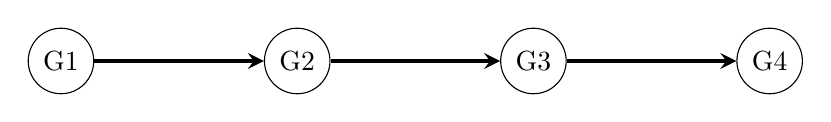
\begin{tikzpicture}
      % Define nodes
      \node[circle, draw] (A) at (0,0) {G1};
      \node[circle, draw] (B) at (3,0) {G2};
      \node[circle, draw] (C) at (6,0) {G3};
      \node[circle, draw] (D) at (9,0) {G4};
      
      % Define edges
      \draw[->, >=stealth, line width=1.5pt] (A) -- (B);
      \draw[->, >=stealth, line width=1.5pt] (B) -- (C);
      \draw[->, >=stealth, line width=1.5pt] (C) -- (D);
    \end{tikzpicture}
    \caption[{[Pla] TD for project definition}]{This graph represents the task dependencies for project definition, self elaborated}
    \label{G_dependences}
\end{figure}

\subsection{Research and Learning \textbf{(RL)}}
In this section is included all the research and learning that I need for the correct development of the project.
Here I will only need access to internet to search for information and access to the different pages and documents that I will be using.
The principal internet resources that I will use are: Royo-Sales et al. \cite{royo_sales_algorithm_2021}, Haskell notes made by Jordi Petit from the subject LP and the Dynamic Pipeline Framework repository.
I may also need to contact my supervisor for Haskell doubts and also Royo-Sales et al. \cite{royo_sales_algorithm_2021} if some critical doubt appears.
This section also have some dependence (\textbf{see Figure \ref{RL_dependences}}) because of the nature of the tasks.
\begin{itemize}
    \item \textbf{RL1} Haskell Refresh \\
        The refresh of my Haskell knowledge and improvement of it. 
        Check for possible libraries and codes \\
        Role: Project Manajer \\
        Expected dedication: 20 hours
    \item \textbf{RL2} TFM assimilation\\
        The reading and understanding of Royo-Sales et al. \cite{royo_sales_algorithm_2021} work. \\
        Role: Researcher \\
        Expected dedication: 25 hours
    \item \textbf{RL3} Dynamic Pipeline Framework \\
        Intensive review of the framework repository. \\
        Role: Haskell Developer \\
        Expected dedication: 30 hours 
\end{itemize}
\begin{figure}[h]
    \centering
    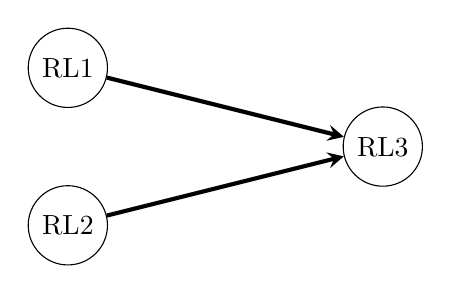
\begin{tikzpicture}
      % Define nodes
      \node[circle, draw] (A) at (0,2) {RL1};
      \node[circle, draw] (B) at (0,0) {RL2};
      \node[circle, draw] (C) at (4,1) {RL3};
      
      % Define edges
      \draw[->, >=stealth, line width=1.5pt] (A) -- (C);
      \draw[->, >=stealth, line width=1.5pt] (B) -- (C);
    \end{tikzpicture}
    \caption[{[Pla] TD for reserch and learning}]{This graph represents the task dependencies for research and learning, self elaborated}
    \label{RL_dependences}
\end{figure}

\subsection{First Algorithm Development \textbf{(FA)}}
This section includes the development of the first algorithm, the one that will be put to test my Haskell knowledge acquired.
Here I will need my personal laptop (as I have the entire environment required) and access to the GitHub repository \cite{forner_gomez_incremental_nodate}.
For all the Haskell doubts I may need to contact my supervisor and for Dynamic pipeline doubts I should contact my co-supervisor as she is the expert.
This task has a linear dependency (\textbf{see Figure \ref{FA_dependences}}), but a critical testing error may need to reimplement some parts of the code, generating a circular dependency.
\begin{itemize}
    \item \textbf{FA1} Algorithm Scaffold \\
        Here will be set the base of the algorithm and the form of the dynamic pipeline.
        Check for possible libraries and codes \\
        Role: Haskell Developer\\
        Expected dedication: 20 hours
    \item \textbf{FA2} Algorithm Implementation\\
        This part is the pure implementation of the algorithm. \\
        Role: Haskell Developer \\
        Expected dedication: 50 hours
    \item \textbf{FA3} Algorithm Testing \\
        Testing of the algorithm implementation, littles changes are also contemplated here (no big changes) \\
        Role: Haskell Developer \\
        Expected dedication: 10 hours 
\end{itemize}
\begin{figure}[h]
    \centering
    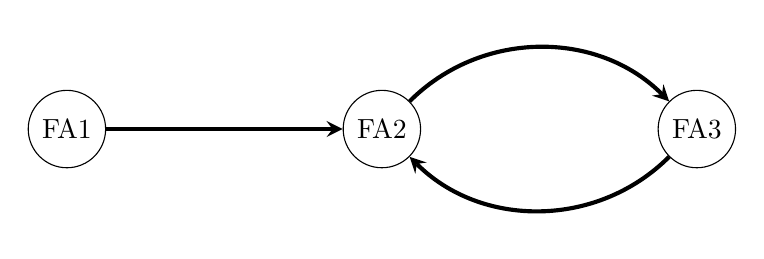
\begin{tikzpicture}
      % Define nodes
      \node[circle, draw] (A) at (0,0) {FA1};
      \node[circle, draw] (B) at (4,0) {FA2};
      \node[circle, draw] (C) at (8,0) {FA3};
      
      % Define edges
      \draw[->, >=stealth, line width=1.5pt] (A) -- (B);
      \draw[->, >=stealth, line width=1.5pt] (B) edge[bend left=45] (C);
      \draw[->, >=stealth, line width=1.5pt] (C) edge[bend left=45] (B);
    \end{tikzpicture}
    \caption[{[Pla] TD for first algorithm development}]{This graph represents the task dependencies for first algorithm development, self elaborated}
    \label{FA_dependences}
\end{figure}

\subsection{Second Algorithm Development \textbf{(SA)}}
This is the final section and the goal of this work, here I will try to improve the original algorithm.
Again, here I will only need my personal laptop and access to internet resources.
This section will need a lot of contact with my supervisor and co-supervisor, specially my co-supervisor, who is the expert in the algorithm.
Here the dependence are similar to the previous section (\textbf{see Figure \ref{SA_dependences}}), as is also a development of an algorithm.
This task is especial, because it is difficult to estimate the exact scope of my project, so maybe I make some improvement and then have more time to repeat this process and make another improvement.
\begin{itemize}
    \item \textbf{SA1} Finding Weak Points \\
        Here I will be looking for possible improvements in the code.\\
        Role: Haskell Developer and Researcher\\
        Expected dedication: 15 hours
        \item \textbf{SA2} Improvement Scaffolds \\
        Here will be set the base for the improvements of the algorithms find in the previous task
        Check for possible libraries and codes \\
        Role: Haskell Developer \\
        Expected dedication: 15 hours
    \item \textbf{SA3} Algorithm Implementation\\
        This part is the pure implementation of the algorithm. \\
        Role: Haskell Developer \\
        Expected dedication: 80 hours
    \item \textbf{SA4} Algorithm Testing \\
        Testing of the algorithm implementation, little changes are also contemplated here (no big changes).
        Here more time is needed in comparation of previous section as the size of the code and algorithm\\
        Role: Haskell Developer \\
        Expected dedication: 20 hours
\end{itemize}
\begin{figure}[h]
    \centering
    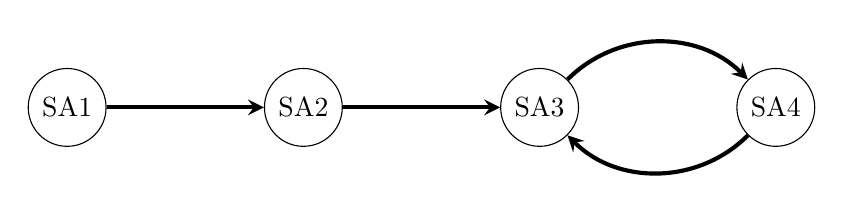
\begin{tikzpicture}
      % Define nodes
      \node[circle, draw] (A) at (0,0) {SA1};
      \node[circle, draw] (B) at (3,0) {SA2};
      \node[circle, draw] (C) at (6,0) {SA3};
      \node[circle, draw] (D) at (9,0) {SA4};
      
      % Define edges
      \draw[->, >=stealth, line width=1.5pt] (A) -- (B);
      \draw[->, >=stealth, line width=1.5pt] (B) -- (C);
      \draw[->, >=stealth, line width=1.5pt] (C) edge[bend left=45] (D);
      \draw[->, >=stealth, line width=1.5pt] (D) edge[bend left=45] (C);
    \end{tikzpicture}
    \caption[{[Pla] TD for second algorithm development}]{This graph represents the task dependencies for second algorithm development, self elaborated}
    \label{SA_dependences}
\end{figure}

\subsection{Documentation \textbf{(D)}}
Finally, this last section is a bit special because it is not planned to be done at the end of the all the previous sections.
It is planned to be done in parallel as the project is developed and the different sections are finished.
Here, all I need is my personal laptop to write all the documentation using \LaTeX.
Here I may need to contact for some help and feedback, but is not mandatory.
There are no direct dependence, but we can consider that we need to complete one section or task before starting to write, so we can consider a graph like shown below (\textbf{see Figure \ref{D_dependences}}).
\begin{itemize}
    \item \textbf{D1} Documentation of RL section \\
        This corresponds to the documentation of the research and learning section. \\
        Role: Project Manager \\
        Expected dedication: 10 hours
    \item \textbf{D2} Documentation of FA section\\
        This corresponds to the documentation of the first algorithm section. \\
        Role: Project Manager \\
        Expected dedication: 20 hours
    \item \textbf{D3} Documentation of SA section \\
        This corresponds to the documentation of the second algorithm section. \\
        Role: Project Manager \\
        Expected dedication: 20 hours
    \item \textbf{D4} Final Documentation \\
    This corresponds to the union of all the previous parts, with the additional parts (conclusions, bibliography, etc.) and the revision of the entire document. \\
    Role: Project Manager \\
    Expected dedication: 50 hours        
\end{itemize}
\begin{figure}[h]
    \centering
    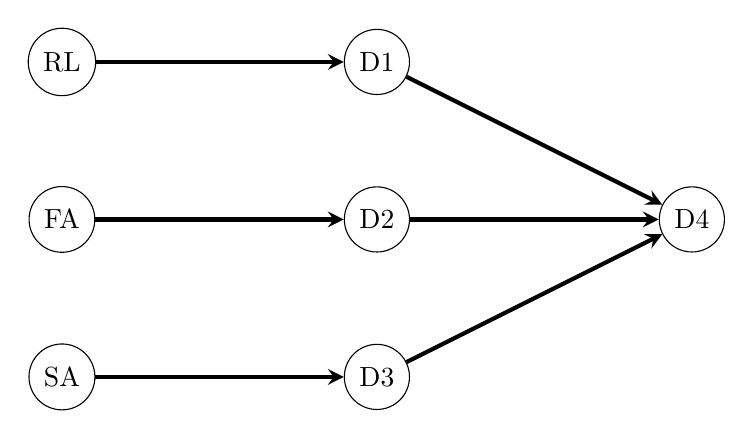
\begin{tikzpicture}
      % Define nodes
      \node[circle, draw] (A) at (4,4) {D1};
      \node[circle, draw] (B) at (4,2) {D2};
      \node[circle, draw] (C) at (4,0) {D3};
      \node[circle, draw] (D) at (8,2) {D4};

      \node[circle, draw] (E) at (0,4) {RL};
      \node[circle, draw] (F) at (0,2) {FA};
      \node[circle, draw] (G) at (0,0) {SA};
      
      % Define edges
      \draw[->, >=stealth, line width=1.5pt] (A) -- (D);
      \draw[->, >=stealth, line width=1.5pt] (B) -- (D);
      \draw[->, >=stealth, line width=1.5pt] (C) -- (D);
      \draw[->, >=stealth, line width=1.5pt] (E) -- (A);
      \draw[->, >=stealth, line width=1.5pt] (F) -- (B);
      \draw[->, >=stealth, line width=1.5pt] (G) -- (C);
    \end{tikzpicture}
    \caption[{[Pla] TD for documentation}]{This graph represents the task dependencies for documentation, self elaborated}
    \label{D_dependences}
\end{figure}

\section{Estimations and Gantt chart}
\subsection{Summary table}
Now that we defined all the tasks, minimum hours and dependence, we can make this following summary table:
\definecolor{LightGray}{rgb}{0.8,0.8,0.8}
\begin{table}[H]
    \begin{adjustwidth}{-1in}{-1in}
    \centering
    \begin{tabular}{|p{5cm}|c|c|p{2cm}|p{3cm}|p{3cm}|}
    \hline
    \textbf{Description} & \textbf{TAG} & \textbf{Hours} & \textbf{Previous Tasks} & \textbf{Requirements} & \textbf{Human Resource} \\
    \hline
    \hline	
    \rowcolor{LightGray}
    \textbf{Project definition and planning} & \textbf{G} & \textbf{75} & \textbf{-} & \textbf{-} & \textbf{-}  \\
    \hline
    Context and Scope & G1 & 20 & Laptop & None & None \\
    \hline
    Planning & G2 & 12 & G1 & Laptop & GEP Tutor \\
    \hline
    Budget and Sustainability & G3 & 18 & G2 & Laptop & GEP Tutor \\
    \hline
    Final Document & G4 & 25 & G3 & Laptop & GEP Tutor \\
    \hline
    \hline
    \rowcolor{LightGray}
    \textbf{Research and Learning} & \textbf{RL} & \textbf{75} & \textbf{G} & \textbf{-} & \textbf{-} \\
    \hline
    Haskell Refresh & RL1 & 20 & None & Laptop, Books & Supervisor \\
    \hline
    TFM assimilation & RL2 & 25 & None & Laptop & Supervisors \\
    \hline
    Dynamic Pipeline Framework & RL3 & 30 & RL1, RL2 & Laptop & Royo-Sales et al. \cite{royo_sales_algorithm_2021} \\
    \hline
    \hline
    \rowcolor{LightGray}
    \textbf{First Algorithm Development} & \textbf{FA} & \textbf{80} & \textbf{RL} & \textbf{-} & \textbf{-} \\
    \hline
    Algortim Scaffold & FA1 & 20 & None & None & Supervisors\\
    \hline
    Algorith Implementation & FA2 & 50 & FA1 & Laptop & Supervisor\\
    \hline
    Algorithm Testing & FA3 & 10 & FA2 & Laptop & None \\
    \hline
    \hline
    \rowcolor{LightGray}
    \textbf{Second Algorithm Development} & \textbf{SA} & \textbf{130} & \textbf{FA} & \textbf{-} & \textbf{-} \\
    \hline
    Finding Weak Points & SA1 & 15 & None & Laptop & Co-supervisor\\
    \hline
    Improvement Scaffolds & SA2 & 15 & SA1 & None & None\\
    \hline
    Algorith Implementation & SA3 & 80 & SA2 & Laptop & Supervisor\\
    \hline
    Algorithm Testing & SA4 & 20 & SA3 & Laptop & None\\
    \hline
    \hline
    \rowcolor{LightGray}
    \textbf{Documentation} & \textbf{D} & \textbf{100} & \textbf{RL,FA,SA,G} & \textbf{-} & \textbf{-} \\
    \hline
    Documentation of RL section & D1 & 10 & RL & Laptop & None \\
    \hline
    Documentation of FA section & D2 & 20 & FA & Laptop & None \\
    \hline
    Documentation of SA section & D3 & 20 & SA & Laptop & None \\
    \hline
    Final Documentation & D4 & 50 & D1, D2, D3 & Laptop & Supervisors \\
    \hline
    \hline
    \rowcolor{LightGray}
    \multicolumn{6}{|c|}{\textbf{Total (G + RL + FA + SA + D): 460 hours}}  \\
    \hline
    \end{tabular}
    \caption[{[Pla] Project planning summary}]{This is a table summary of the project planning, self elaborated}
    \label{TableResume}
    \end{adjustwidth}
\end{table}
\subsection{Gantt chart}

\definecolor{G_Color}{rgb}{1,0,0}
\definecolor{RL_Color}{rgb}{0,1,0}
\definecolor{FA_Color}{rgb}{0,0,1}
\definecolor{SA_Color}{rgb}{1,1,0}
\definecolor{D_Color}{rgb}{0,1,1}

\begin{figure}[H]
    \begin{adjustwidth}{-1in}{-1in}
    \centering
    \begin{ganttchart}[vgrid, hgrid, x unit=0.55cm, y unit chart=0.6cm]{1}{17}
    \gantttitle{Week}{17} \\
    \gantttitlelist{1,...,17}{1} \\
    %SECTION G
    \ganttgroup{G - Project definition and planning [75]}{1}{4} \\ 
    \ganttbar[bar/.style={draw=black, fill=G_Color}] {G1 - Context and Scope [20h]}{1}{1} \\
    \ganttbar[bar/.style={draw=black, fill=G_Color}] {G2 - Planning [12h]}{2}{2} \\
    \ganttbar[bar/.style={draw=black, fill=G_Color}] {G3 - Budget and Sustainability [18h]}{3}{3} \\
    \ganttbar[bar/.style={draw=black, fill=G_Color}] {G4 - Final Document [25h]}{4}{4} \\
    \ganttlink{elem1}{elem2}
    \ganttlink{elem2}{elem3}
    \ganttlink{elem3}{elem4}

    %SECTION RL
    \ganttgroup{RL - Research and Learningt [75]}{5}{7} \\ 
    \ganttbar[bar/.style={draw=black, fill=RL_Color}] {RL1 - Haskell Refresh [20h]}{5}{5} \\
    \ganttbar[bar/.style={draw=black, fill=RL_Color}] {RL2 - TFM assimilation [25h]}{6}{6} \\
    \ganttbar[bar/.style={draw=black, fill=RL_Color}] {RL3 - Dynamic Pipeline Framework [30h]}{7}{7} \\
    \ganttlink{elem0}{elem5}
    \ganttlink{elem6}{elem8}
    \ganttlink{elem7}{elem8}

    %SECTION FA
    \ganttgroup{FA - First Algorithm Development [80]}{8}{10} \\ 
    \ganttbar[bar/.style={draw=black, fill=FA_Color}] {FA1 - Algortim Scaffold [20h]}{8}{8} \\
    \ganttbar[bar/.style={draw=black, fill=FA_Color}] {FA2 - Algorith Implementation [50h]}{9}{10} \\
    \ganttbar[bar/.style={draw=black, fill=FA_Color}] {FA3 - Algorithm Testing [10h]}{10}{10} \\
    \ganttlink{elem5}{elem9}
    \ganttlink{elem10}{elem11}
    \ganttlink{elem11}{elem12}

    %SECTION SA
    \ganttgroup{FA - Second Algorithm Development [130]}{11}{15} \\ 
    \ganttbar[bar/.style={draw=black, fill=SA_Color}] {SA1 - Finding Weak Points [15h]}{11}{11} \\
    \ganttbar[bar/.style={draw=black, fill=SA_Color}] {SA2 - Improvement Scaffolds [15h]}{12}{12} \\
    \ganttbar[bar/.style={draw=black, fill=SA_Color}] {SA3 - Algorith Implementation [80h]}{12}{15} \\
    \ganttbar[bar/.style={draw=black, fill=SA_Color}] {SA4 - Algorithm Testing [20h]}{15}{15} \\
    \ganttlink{elem9}{elem13}
    \ganttlink{elem14}{elem15}
    \ganttlink{elem15}{elem16}
    \ganttlink{elem16}{elem17}
    %SECTION D
    \ganttgroup{D - Documentation [100]}{8}{17} \\
    \ganttbar[bar/.style={draw=black, fill=D_Color}] {D1 - Documentation of RL section [10h]}{8}{10} \\
    \ganttbar[bar/.style={draw=black, fill=D_Color}] {D2 - Documentation of FA section [20h]}{11}{15} \\
    \ganttbar[bar/.style={draw=black, fill=D_Color}] {D3 - Documentation of SA section [20h]}{16}{16} \\
    \ganttbar[bar/.style={draw=black, fill=D_Color}] {D4 - Final Documentation [50h]}{16}{17} \\

    \ganttlink{elem5}{elem19}
    \ganttlink{elem9}{elem20}
    \ganttlink{elem13}{elem21}
    \ganttlink{elem19}{elem22}
    \ganttlink{elem20}{elem22}
    \ganttlink{elem21}{elem22}
    
    \label{GANTT}
    \end{ganttchart}
    \caption[{[Pla] Gantt diagram of the project}]{This is the Gantt diagram of this project, self elaborated}
    \end{adjustwidth}
\end{figure}

\section{Risk management: obstacles and alternatives}
As mentioned in previous sections of this work, there are some potential risks that may appear during the development of the project.
Here will be explained how I will manage them and the alternatives that could be done in case of critical obstacles.
\subsection{Obstacles}
\subsubsection*{Time deadline}
As said previously, this is one of the most important risks of the project. There is not a lot of time, but I have some tools to deal with this problem.
Firstly, the main objective is to obtain more time if needed and my principal activity (and the one that spends more time) is my job as intern.
I have flexibility in my schedule and I can reorganize my week to spend more time in the project.
Also, I have some holidays that I can use to spend more time in the project.
\subsubsection*{Dynamic Pipeline Framework}
I explained that I never used before this framework and I may have some problems with it or it could have some bugs or limitations.
The principal tool to deal with is to contact with his creator, Royo-Sales et al. \cite{royo_sales_algorithm_2021}. Also, I can spend more time studying the framework because I saved some time in case of this obstacle.
This problem could potentially add from 10 to 30 hours to the project.
\subsection{Alternatives}
If some of the previous obstacles appear and I can not deal with them, I could be forced to make some changes in the project.
So the principal alternative is to reduce the scope of the project, reducing the time spent in the last section: the improvement of the algorithm.
This part is the longest of the project and it is planned to be able to be reduced if needed.
It is very comfortable, since I do not need any additional resource and I can adapt it to the time that I have left.

\chapter{Budget and Sustainability}
\section{Budget}
In this section I will identify the costs of the project. 
I will break down the costs into different categories, then I will estimate the costs of each one and finally I will propose a management control system to monitor the costs.
\subsection{Identification of costs}
Here are all the cost group by categories that I will consider in this project.
\subsubsection*{Hardware}
In my project the only hardware that is needed is a computer.
We need a computer for all the process: research, programming, writing the documentation, etc.
If we needed to test our algorithm with a large dataset, we maybe would need a computer with a high performance or a more specialized hardware, but in this work I will not consider this case.
I will consider a generic computer / laptop.
\subsubsection*{Software}
In this project is only planned to use a few software tools.
Starting with the programming language, I will use Haskell.
Haskell has a compiler called Glasgow Haskell Compiler (GHC) and would be sufficient for the project.
I'm also using Visual Studio Code as a text editor, for both writing the code and the documentation.
The next software that I will use is \LaTeX, for writing the documentation.
I also will use GitHub for the version control of the project, that uses Git.
\subsubsection*{Human resources}
Truthy I'm the only human resource that is working in this project, but I will consider me as a person assuming different roles.
As mentinoded in the planning section, I will be taking 3 diferents roles:
\begin{itemize}
    \item Researcher: For tasks RL2, SA1 and some documentation
    \item Haskell Developer: For tasks RL3, all FA tasks and all SA tasks
    \item Project Manager: For all G and D tasks
\end{itemize}
\subsubsection*{Other costs}
I will not consider other costs as the cost of the internet connection, the electricity and the cost of the paper and ink for printing the documentation.
As I consider very specific costs and do not have a huge impact in the total cost.
Other cost that could be considered is the cost of the transportation, cost of the supervisor and co-supervisor work and other stuff that could be needed for the project.
As I consider that these costs are difficult to estimate, I will not consider them in this project.
\subsection{Cost estimates}
Now that all costs are identifies, here I will estimate the cost of each one, considering the duration of the project and the cost of each resource.
\subsubsection*{Hardware}
I will consider a standard price for a good laptop, that is around 1000 euros.
Obviously a laptop have a longer life than the project duration, so I will consider the cost of the laptop as a cost that is distributed in time, amortization.
$$
\text{Amortization} = \text{Laptop Cost} \cdot \frac{\text{Project Duration}}{\text{Laptop Lifespan}}
$$ 
Normaly, laptops have a lifespan of 3 to 5 years with a avegare of 40 hours per week, so I will consider 4 years, 40 hours per week as the lifespan of the laptop. %\cite{}
Also I will consider that the whole project will need the laptop, so there will be a total of 460 hours. 
$$
\text{Amortization} = 1000 \text{€} \cdot \frac{460 \text{hours}}{4 \text{years} \cdot 52 \frac{\text{weeks}}{\text{year}} \cdot 40 \frac{\text{hours}}{\text{week}}} = 55,29 \text{€}
$$
\subsubsection*{Software}
All the software that I will use is free \cite{}. So the total amount of money spend in software will be 0€.
\subsubsection*{Human resources}
I will be tacking the average salary of each role from glassdoor \cite{GlassDoorResearcher} \cite{GlassdoorProjectManager}\cite{GlassdoorSoftwareDeveloper}, a well known website for job search and salary information.
We will check Spain salaries and we will consider 2000 hours per year.
Here we can see the cost of the human resources, assuming a social security multiplier of 1.3.

\begin{table}[H]
    \begin{adjustwidth}{-1in}{-1in} % Adjust margins by -1 inch on both sides
    \centering
    \begin{tabular}{|c|c|c|c|c|}
    \hline
    \textbf{Role} & \textbf{Avg. Salary (€/h)} & \textbf{Hours} & \textbf{Total (€)} & \textbf{Total with Social Security (€)} \\ 
    \hline
    Researcher & 15 & 85 hours & 1275 & 1657.5\\
    \hline
    Haskell Developer & 18 & 200 hours & 3600 & 4680\\
    \hline
    Project Manager & 20 & 175 hours & 3500 & 4550\\
    \hline
    \hline
    \textbf{Total} & 18.2 & 460 & 8375 &  10887.5\\
    \hline
    \end{tabular}
    \caption{Human Resources Cost, self elaborated}
    \label{human_resources}
    \end{adjustwidth}
    \end{table}
\subsubsection*{Risk plan}
Some risks may appear during the project, so I will add some extra money to the budget to cover it.
\begin{enumerate}
    \item Laptop damage: The laptop could be damaged and need to be repaired. I will consider 100€ for this risk.
    \item Extra hours: The project could take more time than expected and each hour of the workers is so expensive. Considering 10 \% more time, gives us 837 €, so I will add 1000€ to the budget.
    \item For other risks and unexpected costs, I will add 10 \% of the total budget, to cover it, 1100 €.
\end{enumerate}
Puting all together, the total amount of money for the unexpected costs is 2037 €.
\subsubsection*{Total budget}
Lets sumarize all the costs and calculate the total budget.
\begin{table}[H]
    \begin{adjustwidth}{-1in}{-1in} % Adjust margins by -1 inch on both sides
    \centering
    \begin{tabular}{|c|c|}
    \hline
    \textbf{Source} & \textbf{Cost (€)} \\ 
    \hline
    Hardware &  55,29 \\
    \hline
    Software & 0 \\
    \hline
    Human Resources & 10887.5 \\
    \hline
    Unexpected & 2037 \\
    \hline
    \hline
    \textbf{Total} & \textbf{12979.79}  \\
    \hline
    \end{tabular}
    \caption{Total budget, self elaborated}
    \label{total_budget}
    \end{adjustwidth}
    \end{table}
\subsection{Management control}
Once we have our budget, I can create a indicator so I can monitor the deviation from the initial plan.
This indicator (C) will be the difference between the expected and actual cost:
$$
C = C_estimado - C_real
$$ 
I can use this indicator both in a general way and with each subsection of the budget, in order to be able to analyze what may be causing a variation in the budget and be able to fix it, either by modifying the budget itself or by restructuring the project.
\section{Sustainability report}
\subsection{Economic Dimension}
After analized my project and made the budget, we can observe that the main cost of the project is the human resources.
Asuming that my plannign is correct, I can confirm that no unnecessary costs are being generated, beacause I'm using free software and the minimun hardware required.
Also this project have the goal of improving an implementation of an algorithm, meaning a possible improvement in the efficiency of the algorithm, which could lead to a reduction in time, which means a reduction of the cost.
\subsection{Environmental Dimension}
As mentioned before, the only environmental impact of the project is the energy consumed by the laptop. 
The energy and impact are minimum, so we can consider this project as environmentally friendly.
Also as previous point, the project could lead to a reduction in time, which means a reduction of the energy consumed.
A good point about projects like mine is that their useful life can be considered 'unlimited'.
This is because it is a research and development project, providing utility at all times.
\subsection{Social Dimension}
In personal terms, I think it will have a great impact on my life and career as a student, since this project will be the first 'big project', which will help me learn from mistakes for future projects.
This project may not have a big social impact, but it can do your part in the world of computing and especially in the world of Haskell programming.

\chapter{Laws and regulations}
Consulting the BOE, law 14/2011, updated on 01/11/2023, article 15 (page 28) tells us about various obligations of the researcher and here I will comment on those that involve me \cite{}
\begin{itemize}
    \item \textbf{Avoid plagiarism and misappropriation of authorship of scientific works or third-party technologies} \\
    On this point, I have at all times cited other people's resources and whenever I have used a third-party technological resource I have made sure that it is open source and that its necessary citations are made.
    \item \textbf{Inform the entities for which it provides services of all the findings, discoveries and results susceptible to legal protection, and collaborate in the processes of protection and transfer of the results of their investigations} \\
    At all times I have been in contact with my director and have been reporting on my work.
    \item \textbf{Disseminate the results of your investigations, if applicable, as indicated in this law, so that the results are used through communication and transfer to other research, social or technological contexts, and if applicable, for their marketing and valuation. In particular, the research staff must ensure and take the initiative so that its results generate social value} \\
    This work will be public once finished and everyone will be able to take advantage of the discoveries.
    \item \textbf{Ensure that your work is relevant to society} \\
    This work can help expand resources on dynamic pipeline and Haskell code.
    \item \textbf{Use the name of the entities for which you provide services in the realization of its scientific activity, in accordance with the internal regulations of said entities and the agreements, pacts and conventions that they subscribe} \\
    On the cover of this work you will find at all times the name of the entity (UPC) and the faculty (FIB) as well as their logos. 
    \item \textbf{Adopt the necessary measures to comply with the applicable regulations in matters of data protection and confidentiality} \\
    At all times, we are ensuring compliance with data protection, always using data that is free to use and that complies with the laws.
\end{itemize}
\chapter{Updates}
\section{Updates respect initial planning}
\subsection{About tasks and time planification}
\subsubsection*{Changes}
Regarding the initial planning of the project, there have not been very big changes.
The main change has been that I have needed more investment of time in understanding the library and in coding the word counting problem.
This is because I have found the need to make several adaptations to the library to allow more options and be able to implement my initial problem.
Everything and so I have only needed 2 extra week in the overall time of the \textbf{RL} and \textbf{FA} sections.

In addition to this, I have been able to specify with Edelmira what improvements I can make to the library.
This process was also planned for later, so it also changes the planning a bit.

\subsubsection*{Consequences}
All these changes in planning mean that there is less time left to perform the following tasks (SA, D3, D4).
But at the same time I have invested more time getting to know the library and programming, so I foresee that it will take me less time to improvements to the library that Edelmira proposes. 

\subsubsection*{New planning}
With this updates, the new planning is as follows:
\newpage

\definecolor{LightGray}{rgb}{0.8,0.8,0.8}
\begin{table}[H]
    \begin{adjustwidth}{-1in}{-1in}
    \centering
    \begin{tabular}{|p{5cm}|c|c|p{2cm}|p{3cm}|p{3cm}|}
    \hline
    \textbf{Description} & \textbf{TAG} & \textbf{Hours} & \textbf{Previous Tasks} & \textbf{Requirements} & \textbf{Human Resource} \\
    \hline
    \hline	
    \rowcolor{LightGray}
    \textbf{Project definition and planning} & \textbf{G} & \textbf{75} & \textbf{-} & \textbf{-} & \textbf{-}  \\
    \hline
    Context and Scope & G1 & 20 & Laptop & None & None \\
    \hline
    Planning & G2 & 12 & G1 & Laptop & GEP Tutor \\
    \hline
    Budget and Sustainability & G3 & 18 & G2 & Laptop & GEP Tutor \\
    \hline
    Final Document & G4 & 25 & G3 & Laptop & GEP Tutor \\
    \hline
    \hline
    \rowcolor{LightGray}
    \textbf{Research and Learning} & \textbf{RL} & \cancel{\textcolor{red}{75}} 95 & \textbf{G} & \textbf{-} & \textbf{-} \\
    \hline
    Haskell Refresh & RL1 & 20 & None & Laptop, Books & Supervisor \\
    \hline
    TFM assimilation & RL2 & \cancel{\textcolor{red}{25}} 15& None & Laptop & Supervisors \\
    \hline
    Dynamic Pipeline Framework & RL3 & \cancel{\textcolor{red}{30}} 60 & RL1, RL2 & Laptop & Juan Pablo \\
    \hline
    \hline
    \rowcolor{LightGray}
    \textbf{First Algorithm Development} & \textbf{FA} & \cancel{\textcolor{red}{80}} \textbf{100}  & \textbf{RL} & \textbf{-} & \textbf{-} \\
    \hline
    Algortim Scaffold & FA1 & 20 & None & None & Supervisors\\
    \hline
    Algorith Implementation & FA2 & \cancel{\textcolor{red}{50}} 70 & FA1 & Laptop & Supervisor\\
    \hline
    Algorithm Testing & FA3 & 10 & FA2 & Laptop & None \\
    \hline
    \hline
    \rowcolor{LightGray}
    \textbf{Second Algorithm Development} & \textbf{SA} & \cancel{\textcolor{red}{130}} \textbf{90}  & \textbf{FA} & \textbf{-} & \textbf{-} \\
    \hline
    Finding Weak Points & SA1 & \cancel{\textcolor{red}{15}} 10 & None & Laptop & Co-supervisor\\
    \hline
    Improvement Scaffolds & SA2 & \cancel{\textcolor{red}{15}} 10 & SA1 & None & None\\
    \hline
    Algorith Implementation & SA3 & \cancel{\textcolor{red}{80}} 50 & SA2 & Laptop & Supervisor\\
    \hline
    Algorithm Testing & SA4 & 20 & SA3 & Laptop & None\\
    \hline
    \hline
    \rowcolor{LightGray}
    \textbf{Documentation} & \textbf{D} & \textbf{100} & \textbf{RL,FA,SA,G} & \textbf{-} & \textbf{-} \\
    \hline
    Documentation of RL section & D1 & 10 & RL & Laptop & None \\
    \hline
    Documentation of FA section & D2 & 20 & FA & Laptop & None \\
    \hline
    Documentation of SA section & D3 & 20 & SA & Laptop & None \\
    \hline
    Final Documentation & D4 & 50 & D1, D2, D3 & Laptop & Supervisors \\
    \hline
    \hline
    \rowcolor{LightGray}
    \multicolumn{6}{|c|}{\textbf{Total (G + RL + FA + SA + D): 460 hours}}  \\
    \hline
    \end{tabular}
    \caption[{[Upt] New project planning summary}]{This is a table summary of the new project planning, self elaborated}
    \label{TableResume2}
    \end{adjustwidth}
\end{table}

\subsection{About scope}
\subsubsection*{Changes}
Since initially planning the scope of my work, I have had to modify it as I have progressed.
The reason is that when working with the Haskell library, I have encountered some lack of functionality at some points.
I have found that Juan Pablo made a very complete library but a little oriented to his work.
That's why when trying to implement the word counting problem, I have had to expand and create new functionalities. 

\subsubsection*{Consequences}
No several consequences have been derived from this change.
Just that I have had to invest more time in understanding the library, as reflected in the previous section.
\subsection{About budget}
\subsubsection*{Changes}
Because the scope and time planification changes, budged has also changed. 
The human resource budged needs to be recalculated tacking into account the new time planification. 
The other sections of the budget like hardware, software and unexpected const remain the same.
\subsubsection*{Consequences}
As we can apreciete in the table below, the new human resource budget is less that 0,5\% higher than the initial budget, so the changes are not significant. 
\subsubsection*{New Budget} 
\begin{table}[H]
    \begin{adjustwidth}{-1in}{-1in} % Adjust margins by -1 inch on both sides
    \centering
    \begin{tabular}{|c|c|c|c|c|}
    \hline
    \textbf{Role} & \textbf{Avg. Salary (€/h)} & \textbf{Hours} & \textbf{Total (€)} & \textbf{Total with Social Security (€)} \\ 
    \hline
    Researcher & 15 & \cancel{\textcolor{red}{85}} 75 hours & \cancel{\textcolor{red}{1275}} 1125 & \cancel{\textcolor{red}{1657.5}} 1462.5\\
    \hline
    Haskell Developer & 18 & \cancel{\textcolor{red}{200}} 210 hours & \cancel{\textcolor{red}{3600}} 3780 & \cancel{\textcolor{red}{4680}} 4914\\
    \hline
    Project Manager & 20 & 175 hours & 3500 & 4550\\
    \hline
    \hline
    \textbf{Total} & \cancel{\textcolor{red}{18.2}} 18.3 & 460 & \cancel{\textcolor{red}{8375}} 8405 & \cancel{\textcolor{red}{10887.5}} 10926.5\\
    \hline
    \end{tabular}
    \caption[{[Upt] New human resources costs}]{This is a table summary of the new human resources costs, self elaborated}
    \label{new_human_resources}
    \end{adjustwidth}
\end{table} 

\begin{table}[H]
    \begin{adjustwidth}{-1in}{-1in} % Adjust margins by -1 inch on both sides
    \centering
    \begin{tabular}{|c|c|}
    \hline
    \textbf{Source} & \textbf{Cost (€)} \\ 
    \hline
    Hardware &  55,29 \\
    \hline
    Software & 0 \\
    \hline
    Human Resources & \cancel{\textcolor{red}{10887.5}} 10926.5 \\
    \hline
    Unexpected & 2037 \\
    \hline
    \hline
    \textbf{Total} & \cancel{\textcolor{red}{12979.79}} \textbf{13018.79}  \\
    \hline
    \end{tabular}
    \caption[{[Upt] New final budget}]{This is a table summary of the new total budget, self elaborated}
    \label{new_total_budget}
    \end{adjustwidth}
\end{table}
\chapter{Improving the dynamic pipeline library} \label{IDPL}
In this chapter, we will understand and learn how to use the Haskell DynamicPipeline library developed by Juan Pablo Royo Sales.
To do this, we will carry out a small analysis and try to implement the small 'toy problem' of counting words.
Finally, with all the knowledge acquired, we will try to improve the library, updating it to the new functionalities of the most modern Haskell and adding functionalities to it. 
\section{Introduction}
To properly understand the library, we must first understand how the DynamicPipeline paradigm works.
This work will not provide an extensive explanation of the library, as it is not within the scope of this thesis and a general understanding is sufficient.
For a more detailed explanation, please refer to the work of Juan Pablo Royo Sales.
\subsection*{Dynamic Pipeline Paradigm}
As mentioned at the beginning of this work, the dynamic pipeline paradigm is a computational model based on a chain of stages.
We can define the structure of a Dynamic Pipeline from four types of stages: the Source (Sr), the Sink (Sk), the Generator (G), and the Filter (F).
Defining the behavior of these four stages of the pipeline is sufficient to define the behavior of the entire pipeline. \\

The different stages are connected to each other by a non-zero number of channels.
Initially, the pipeline consists of a Sr, which is connected by channels to the G, which is also connected by channels to the Sk.
During execution, the G is responsible for generating Fs, which are placed between the Sr and the G, connecting the channels of the Sr to the first F and the last F to the G.
These would be some examples of states of a Dynamic Pipeline:

\begin{figure}[H]
    \centering
    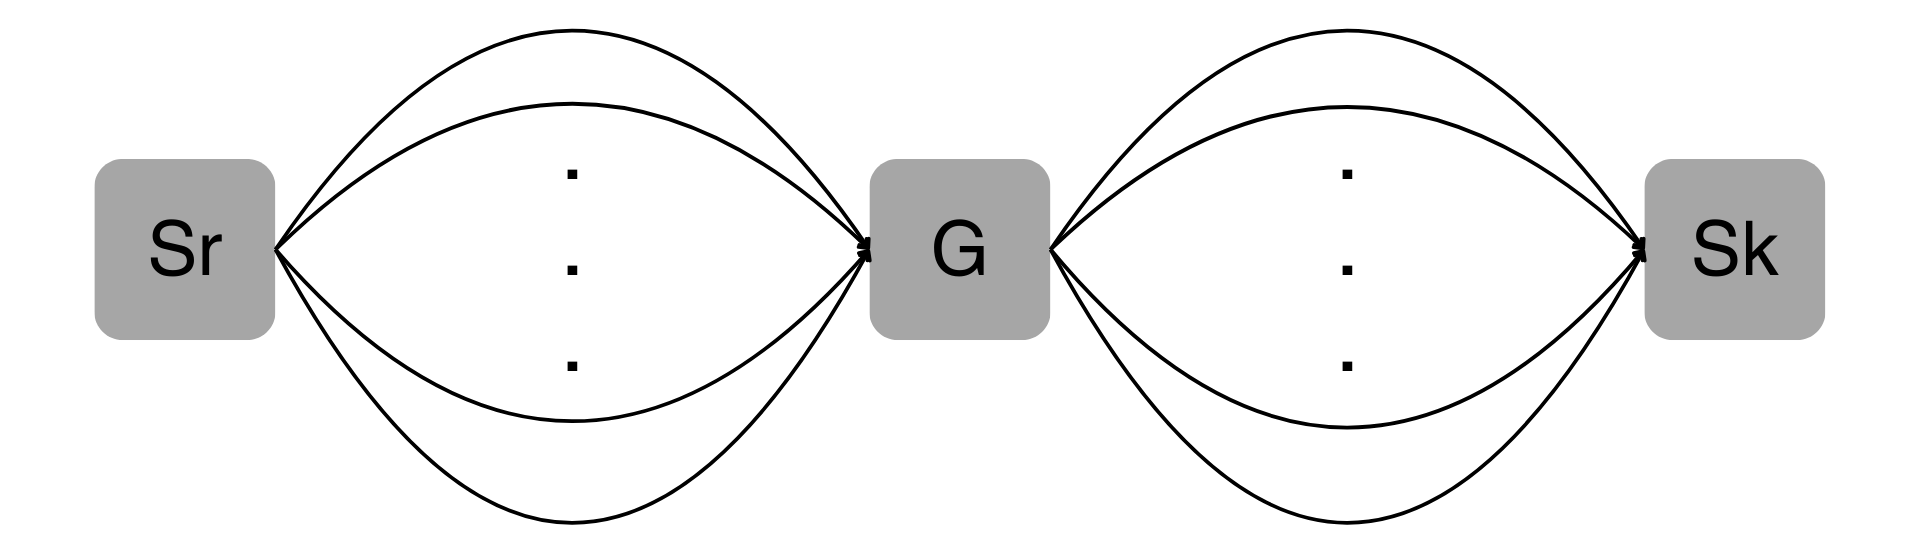
\includegraphics[width=1\textwidth]{DP100.png}
    \caption[{[Lib] Initia structure of a DP}]{This is the initial structure of a Dynamic Pipeline, self-made with Canva}
    \label{fig:DP100}
\end{figure}

\begin{figure}[H]
    \centering
    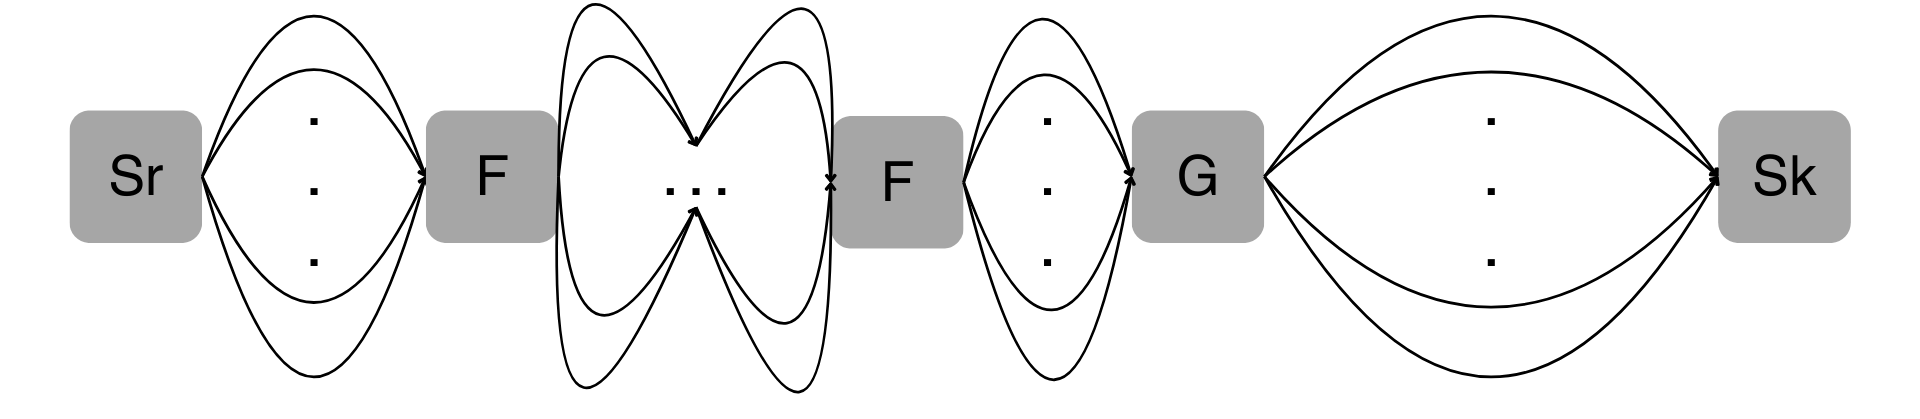
\includegraphics[width=1\textwidth]{DP101.png}
    \caption[{[Lib]} Posible structure of a DP]{This is a posible state of a Dynamic Pipeline, self-made with Canva}
    \label{fig:DP101}
\end{figure}

\subsection*{Source and Sink}
These two stages are the easiest to define and understand.
The Source and the Sink are responsible for introducing the input stream into the Pipeline and collecting the results and output them, respectively.
The Sr takes as input any form of data stream and is responsible for filling the different channels of the pipeline with data, which may already be processed and adapted by the stage itself.
At the end of the pipeline, the Sk is responsible for reading the different channels and returning the output to the outside.

\subsection*{Generator}
The Generator is more sophisticated and complex.
For each element it processes, it must decide whether to let it continue to the Sk and thus pass to the output or not.
In addition, it is responsible for deciding when to generate a Filter and add it to the pipeline.
For each element it reads, it can decide whether or not to generate a Filter, which is interposed between the last generated F (or the Sr if it is the first generated F) and itself.
It is also responsible for initializing the Filter by giving it a value for its parameter and its state.

\subsection*{Filter}
The last stage is the Filter.
It is the heart of the pipeline's computation and is responsible for processing and treating the data.
Each F has a state, which can be updated, and a parameter.
The execution of each filter is made up of a set of actors, which can be understood as the minimum unit of computation.
Each actor can consult the filter's parameter and state and update the latter.
It can also decide whether to pass on the data it processes and even generate new data to pass through the pipeline.
The actors are executed sequentially, one after the other, from the first to the last.

\section{Dynamic Pipeline Library}
Once we understand the basics of the Dynamic Pipeline paradigm, we can move on to review the library developed by Juan Pablo.
The first thing we can observe about the Haskell library is that it provides a set of types to work comfortably.
In general, there is one type for each concept of the dynamic pipeline (Sr, G, Sk, Channel, Actor, ...):

\begin{figure}[H]
    \begin{tabular}{c}
        \begin{lstlisting}
data Sink
data Generator (a :: Type), a (*$\sim$*) Channel
data Source (a :: Type), a (*$\sim$*) Channel
data FeedbackChannel (a :: Type), a (*$\sim$*) Channel
data Channel (a :: Type), a (*$\sim$*) (Type :<+> ... :<+> Eof)
data DynamicPipeline dpDef filtStat filterParam st, 
     dpDef (*$\sim$*) Source (Channel ..):=> 
                    Generator(Channel ..):=>Sink
data a :=> b, a & b (*$\sim$*) Stage
        \end{lstlisting}
    \end{tabular}
    \caption[{[Code]}Library data types]{These are some data types provided by the library}
    \label{fig:HC1}
\end{figure}

Based on these initial type definitions, we can see that the library provides us with the mecanism to define the DynamicPipeline type, which will determine the structure of our pipeline.
We can observe that it starts with an Sr that has a set of homogeneous type channels connected to a G, which is also connected to the end of the pipeline Sk through homogeneous type channels. \\

The library also introduces the concept of a Feedback Channel, which is a channel that allows feedback from the Generator (G) back into the pipeline.
This means that we can optionally add an additional stage with the sole task of feeding processed data back to the Source (Sr).
We will delve deeper into this topic later.

\subsection{Library combinators}
The library also provides a set of combinators (functions) for creating the different stages (Sr, G, Sk, and F).
The syntax of these functions can be quite complex, making them difficult to understand.
Since the goal of my work is not to fully comprehend the library and the underlying Haskell grammar, I will instead focus on explaining the concept of these functions and how to use them in a more straightforward manner.
This will enable anyone with a basic understanding of Haskell to implement their own Dynamic Pipeline for their specific problem.

\begin{figure}[H]
    \begin{tabular}{c}
        \begin{lstlisting}
withSource :: Stage (WithSource dpDef (DP st))
withGenerator :: Stage (WithGenerator dpDef filter (DP st))
withSink :: Stage (WithSink dpDef (DP st))
        \end{lstlisting}
    \end{tabular}
    \caption[{[Code]}Library combinators]{Some combinators provided by the library}
    \label{fig:HC2}
\end{figure}
Let's break down each combinator to understand how to use it to achieve the desired result.

\subsubsection*{Combinator withSource}

The withSource combinator is used to create a Source stage.
It takes a function as input (we will refere as fillChannels), which is responsible for filling the Source stage's output channels for any tipe of input.
This function receives the output channels of the Sr stage that are conected to G (or F) as arguments and should send data to these channels.

\begin{figure}[H]
    \begin{tabular}{c}
        \begin{lstlisting}
source :: Stage(   WriteChannel (*$t_1$*)
                -> WriteChannel (*$t_2$*)
                        .
                        .
                        .
                -> WriteChannel (*$t_n$*)
                -> DP st ()
                )
source = withSource @DPStructure . fillChannels

fillChannels ::WriteChannel (*$t_1$*)
            -> WriteChannel (*$t_2$*)
                    .
                    .
                    .
            -> WriteChannel (*$t_n$*)
            -> DP st ()
fillChannels (*$w_1$*) ... (*$w_n$*) = ...
        \end{lstlisting}
    \end{tabular}
    \caption[{[Code]}withSource combinator]{Function to get a Source stage using withSource combinator}
    \label{fig:HC3}
\end{figure}

Alright, this should be enough to create our Source stage.
We simply need to implement the fillChannels function to fill the different channels.
For this purpose, the library provides helper functions that simplify filling a channel from an input source (such as an array or a file).

\begin{figure}[H]
    \begin{tabular}{c}
        \begin{lstlisting}
--Feed a WriteChannel froma a Monadic Seed
unfoldM :: MonadIO m	 
        => m a	    --Monadic seed
        -> (a -> b) --Map input a to WriteChannel type b
        -> m Bool	--When stop unfolding
        -> WriteChannel b   --WriteChannel to feed	
        -> m () 

--Feed a WriteChannel from a file
unfoldFile :: MonadIO m	 
            => FilePath	          --FilePath to read from
            -> WriteChannel b     --WriteChannel to feed
            -> (ByteString -> b)  --Map ByteString to type b
            -> m ()

--Feed a WriteChannel from a foldable (like array)
unfoldT :: (MonadIO m, Foldable t) 
            => t a            --Foldable to unfold
            -> WriteChannel b --WriteChannel to feed
            -> (a -> b) --Map input a to WriteChannel type b
            -> m ()
        \end{lstlisting}
    \end{tabular}
    \caption[{[Code]}Fead channels]{Functions provided by library to fead channels}
    \label{fig:HC4}
\end{figure}

\subsubsection*{Combinator withSink}
Similar to withSource, the withSink combinator is used to create a Sink stage.
It takes a function as input (we will refere as readChannels), which is responsible for reading the Sink stage's input channels to output it.
This function receives the input channels coming from G as arguments and should output the results.

\begin{figure}[H]
    \begin{tabular}{c}
        \begin{lstlisting}
sink   :: Stage(   ReadChannel (*$t_1$*)
                -> ReadChannel (*$t_2$*)
                        .
                        .
                        .
                -> ReadChannel (*$t_n$*)
                -> DP st ()
                )
sink = withSink @DPStructure . readChannels

readChannels ::ReadChannel (*$t_1$*)
            -> ReadChannel (*$t_2$*)
                    .
                    .
                    .
            -> ReadChannel (*$t_n$*)
            -> DP st ()
readChannels (*$r_1$*) ... (*$r_n$*) = ...
        \end{lstlisting}
    \end{tabular}
    \caption[{[Code]}withSink]{Function to get a Sink stage using withSink combinator}
    \label{fig:HC5}
\end{figure}

With this steps, similar to withSource, should be enough to create our Sink stage.
We simply need to implement the readChannels function to output the results.
For this purpose, the library do not provide much help, we have just a function to read a channel and fill a generic output.

\begin{figure}[H]
    \begin{tabular}{c}
        \begin{lstlisting}
--Read a ReadChannel and fold it with a monadic function
foldM_ :: MonadIO m	 
        => ReadChannel a --ReadChannel to read
        -> (a -> m ())  --Computation to do with read element
        -> m ()
        \end{lstlisting}
    \end{tabular}
    \caption[{[Code]}Read channels]{Functions provided by library to read channels}
    \label{fig:HC6}
\end{figure}

\subsubsection*{Combinator withGenerator}
Finally, we have the withGenerator combinator, which is similar to the previous two but with some additional nuances.
As we recall, the G stage has both input and output channels, and it is also responsible for generating F stages.
Therefore, it must determine which of the read data should be passed to the output channels and what conditions must be met to generate an F stage.

The withGenerator combinator takes a function as input, which we will refer to as the genAction function.
This function is responsible for handling all the tasks mentioned above.

\begin{figure}[H]
    \begin{tabular}{c}
        \begin{lstlisting}
generator :: Stage(Filter DPExample filtStat filtPar st
                -> ReadChannel (*$t_1$*)
                        .
                        .
                        .
                -> ReadChannel (*$t_n$*)
                -> WriteChannel (*$t_1$*)
                        .
                        .
                        .
                -> WriteChannel (*$t_n$*)
                -> DP st ()
                )
generator = withGenerator @DPStructure . genAction

genAction ::   Filter DPExample filtStat filtPar st   
            -> ReadChannel (*$t_1$*)
                    .
                    .
                    .
            -> ReadChannel (*$t_n$*)
            -> WriteChannel (*$t_1$*)
                    .
                    .
                    .
            -> WriteChannel (*$t_n$*)
            -> DP st ()
genAction filter (*$r_1$*) ... (*$r_n$*) (*$w_1$*) ... (*$w_n$*) = ...
        \end{lstlisting}
    \end{tabular}
    \caption[{[Code]} withGenerator]{Function to get a Generator stage using withGenerator combinator}
    \label{fig:HC7}
\end{figure}

To create our G stage, we simply need to implement the genAction function.
The library provides helper functions that can simplify this task:

\begin{figure}[H]
    \begin{tabular}{c}
        \begin{lstlisting}
--Read a ReadChannel and fold it with a monadic function
unfoldF::UnFoldFilter dpDef readElem st filtStat filtPar l	
        -> DP st (HList l)

mkUnfoldFilter :: 
(readElem -> Bool)  --For each element determine if 
                    --interpose a new Filter
-> (readElem -> DP st ()) --For each element that the Filter 
                    --is consuming allow to do something 
                    --outside the filter with that element.
-> Filter dpDef filtStat filterParam st   --Filter Template
-> (readElem -> filtStat) --How to Initiate Internal
                             --Filter StateT (Memory)
-> ReadChannel readElem --Main ReadChannel to feed filter
-> HList l --Rest of the ReadChannels if there are needed
           --(HNil if it only contians 1)
-> UnFoldFilter dpDef readElem st filtStat filterParam l
        \end{lstlisting}
    \end{tabular}
    \caption[{[Code]} unfoldF and mkUnfoldFilter]{Functions unfolF and mkUnfoldFilter that help to implement genAction}
    \label{fig:HC8}
\end{figure}
By composing these two functions, we can generate our G stage.
The library also provides some variations of the mkUnfoldFilter function for easier use (see functions mkUnfoldFilter', mkUnfoldFilterForAll, mkUnfoldFilterForAll').
\subsection{Library smart constructors}
The next set of functions provided by the library to complete our Dynamic Pipeline implementation are Smart Constructors.
In Haskell, a smart constructor is a function that allows us to generate a result in a controlled manner and apply restrictions.
Using them ensures that we meet the necessary conditions and invariants for the correct operation of the pipeline.
\subsubsection*{mkFilter Smart Constructor}
The first smart constructor function provided by the library is mkFilter.
This function allows us to define a F stage with a single actor (logical unit).

\begin{figure}[H]
    \begin{tabular}{c}
        \begin{lstlisting}
filterTemp :: Filter dpDef filtStat filterParam st
filterTemp = mkFilter actor1

actor1 :: filterParam
        -> ReadChannel (*$t_1$*)
                .
                .
                .
        -> ReadChannel (*$t_n$*)
        -> WriteChannel (*$t_1$*)
                .
                .
                .
        -> WriteChannel (*$t_n$*)
        -> StateT filtStat (DP st) ()
actor_1 par (*$r_1$*) ... (*$r_n$*) (*$w_1$*) ... (*$w_n$*) = ...
        \end{lstlisting}
    \end{tabular}
    \caption[{[Code]} mkFilter and actors]{mkFilter smart constructor with definition of an actor}
    \label{fig:HC9}
\end{figure}

Similar to the previous functions, we only need to provide the implementation of the actor of F.
Within this function, we have to determine what to do with each element it processes and decide whether to update the state of F, which elements to pass to the next filters, ...
Here are some functions to perform most of the actions mentioned previously:

\begin{figure}[H]
    \begin{tabular}{c}
        \begin{lstlisting}
-- Push element a into WriteChannel
push :: MonadIO m 
        => a 
        -> WriteChannel a 
        -> m ()

-- Pull element Maybe a from ReadChannel
pull :: MonadIO m 
        => ReadChannel a 
        -> m (Maybe a)

-- Fetch the current value of the state within the monad
get :: Monad m 
    => StateT s m s

-- Sets the state within the monad to s
put :: Monad m 
    => s 
    -> StateT s m ()
        \end{lstlisting}
    \end{tabular}
    \caption[{[Code]}Building actors]{Some functions to implemet the actors}
    \label{fig:HC10}
\end{figure}

It should also be noted that filters can have more than one actor.
The library provides two functions for creating filters with N actors:

\begin{figure}[H]
    %\centering
    \begin{tabular}{c}
        \begin{lstlisting}
-- Add a new Actor to an already existing Filter.
(|>>>) :: Actor dpDef filtStat filterParam 
                (StateT filtStat (DP st))
        -> Filter dpDef filtStat filterParam st	
        -> Filter dpDef filtStat filterParam st

-- Given 2 Actors build a Filter.
(|>>) :: Actor dpDef filtStat filterParam 
                (StateT filtStat (DP st))
    -> Actor dpDef filtStat filterParam 
                (StateT filtStat (DP st))	
    -> Filter dpDef filtStat filterParam st       
        \end{lstlisting}
    \end{tabular}
    \caption[{[Code]} Building filters]{Function to create a filter with N actors}
    \label{fig:HC11}
\end{figure}

\subsubsection*{mkGenerator Smart Constructor}
This second smart constructor allows us to link our definition of G with our definition of F.
Simply passing our 2 previously defined functions as arguments to the function, we obtain a stage that encompasses our 2 definitions and combines them:
\begin{figure}[H]
    %\centering
    \begin{tabular}{c}
        \begin{lstlisting}
mkGenerator :: Stage (WithGenerator dpDef 
             (Filter dpDef filtStat filterParam st) (DP st))	
            -> Filter dpDef filtStat filterParam st	
            -> GeneratorStage dpDef filtStat filterParam st
            
generatorStage::GeneratorStage dpDef filtStat filterParam st
generatorStage = mkGenerator generator filterTemp
        \end{lstlisting}
    \end{tabular}
    \caption[{[Code]}mkGenerator ]{mkGenerator combinator}
    \label{fig:HC12}
\end{figure}

\subsubsection*{mkDP Smart Constructor}
This is the final combiner. It takes the three previously defined definitions (source, sink, generatorStage) and combines them to obtain our dynamic pipeline.
\begin{figure}[H]
    %\centering
    \begin{tabular}{c}
        \begin{lstlisting}
mkDP :: Stage (WithSource dpDef (DP st))	
    -> GeneratorStage dpDef filtStat filterParam st	
    -> Stage (WithSink dpDef (DP st))	
    -> DP st ()

DP' :: DP st ()
DP' = mkDP source generatorStage sink
        \end{lstlisting}
    \end{tabular}
    \caption[{[Code]} mkDP]{mkDP combinator}
    \label{fig:HC13}
\end{figure}
\subsection{Conclusions}
With all of this, we have all the elements to execute our Dynamic Pipeline.
The library give us a function that, given a pipeline, run it to final output result.
\begin{figure}[H]
    \begin{tabular}{c}
        \begin{lstlisting}
runDP :: DP st () 
        -> IO a
    
main :: IO ()
main = runDP DP'
        \end{lstlisting}
    \end{tabular}
    \caption[{[Code]} runDP]{runDP function for runing a DP}
    \label{fig:HC14}
\end{figure}

In this section, we have reviewed the entire library to extract the key concepts and tools necessary to implement the vast majority of Dynamic Pipelines.
We have observed how, using the functions provided by the library, it is only necessary to implement a few basic functions corresponding to the essential functionalities of the pipeline itself.
In this way, anyone with a Dynamic Pipeline algorithm can implement it with just some basic Haskell notions. \\

Here is a summary of the functions to implement for each pipeline:

\begin{figure}[H]
    %\centering
    \begin{tabular}{c}
        \begin{lstlisting}
-- Function defining what we put in each channel
fillChannels ::WriteChannel (*$t_1$*)
            -> WriteChannel (*$t_2$*)
                    .
                    .
                    .
            -> WriteChannel (*$t_n$*)
            -> DP st ()

-- Function defining what we do with the final data
readChannels ::ReadChannel (*$t_1$*)
            -> ReadChannel (*$t_2$*)
                    .
                    .
                    .
            -> ReadChannel (*$t_n$*)
            -> DP st ()


genAction ::   Filter DPExample filtStat filtPar st   
            -> ReadChannel (*$t_1$*)
                    .
                    .
                    .
            -> ReadChannel (*$t_n$*)
            -> WriteChannel (*$t_1$*)
                    .
                    .
                    .
            -> WriteChannel (*$t_n$*)
            -> DP st ()

-- Function defining an actor of a filter
actorN :: filterParam
        -> ReadChannel (*$t_1$*)
                .
                .
                .
        -> ReadChannel (*$t_n$*)
        -> WriteChannel (*$t_1$*)
                .
                .
                .
        -> WriteChannel (*$t_n$*)
        -> StateT filtStat (DP st) ()
        \end{lstlisting}
    \end{tabular}
    \caption[{[Code]}Functions summary]{Functions to implement for a DP}
    \label{fig:HC15}
\end{figure}

\section{Implementing the toy problem}
At this point, we have understood the two fundamental aspects: how a dynamic pipeline works and how to define and implement one.
In this section, we will walk through the entire process of defining and implementing a dynamic pipeline using a toy problem.
The goal is to present an example and obtain a template for future implementations of different problems.
\subsection{Algorithm Definition}
The task at hand is to implement a word counting algorithm using a dynamic pipeline.
The goal is to incrementally process a stream of characters, counting the occurrences of each word, and printing partial results whenever a period ('.') character is encountered.
This approach leverages the incremental nature of dynamic pipelines to provide real-time updates. \\

I will not delve deeply into the process of designing the algorithm itself, as the idea is to focus on the implementation.
Therefore, I will explain my proposed solution for the problem and carry out a small test run to understand the behavior.
To keep my design simple, it will only have one channel, and the filters will only have one actor.
This will minimize the complexity of understanding. Since we only have one channel, the data type that will flow will be tuples (Word, Int).
This will represent a specific word along with its count of how many times it appears.
It should be noted that since there is only one channel, the input data and the data generated by the filters themselves (solutions) will go on the same channel, so a rule will have to be created to differentiate them.

\subsubsection*{Source}
Alright, in our case, the Sr will need to obtain the words from the stream and feed the channel with tuples (Word, Int).
Since these are the input elements, we will initialize the tuple with (Word, 0).
This way, we can differentiate the input data from the solutions (since we know that the solutions will have at least a count of 1).

\begin{figure}[H]
    \centering
    
\includegraphics[width=1\textwidth]{DP102.png}
    \caption[{[Lib]} Source stage]{Grafic representation of the Source stage}
    \label{fig:DP102}
\end{figure}

\subsubsection*{Sink}
This stage is the simplest, as it only has to collect the results and display them.
The Sk will receive tuples (Word, Int) and should display them (to the console or a file, for example) in the desired format.

\begin{figure}[H]
    \centering
    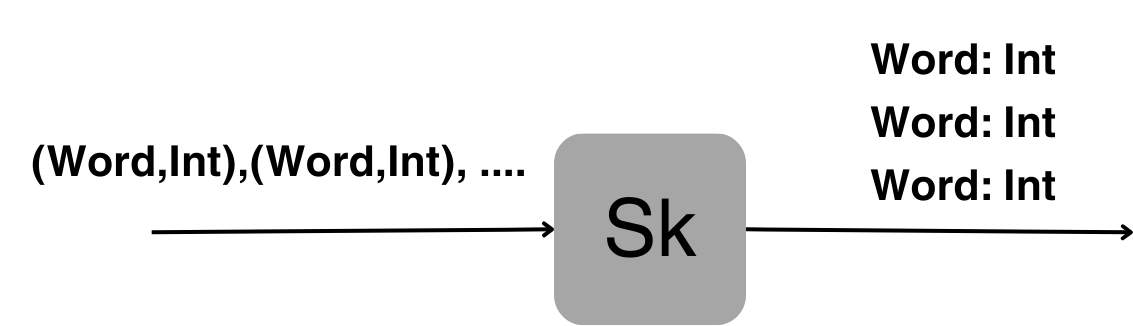
\includegraphics[width=1\textwidth]{DP103.png}
    \caption[{[Lib]} Sink stage]{Grafic representation of the Sink stage}
    \label{fig:DP103}
\end{figure}

\subsubsection*{Generator}
Now let's move on to the heart of the pipeline, the Generator.
This takes care of several tasks, so let's go through them one by one:

\begin{itemize}
    \item \textbf{Create Filters:} For each element it reads, it must decide whether or not to create a F.
    For our problem, the most sensible thing would be to have one filter for each unique word, so the G must ensure that it does not create two filters for the same word.
    To do this, we can take advantage of the fact that filters can also decide not to let words pass.
    We can leave the responsibility of not letting repeated words pass to the filters and have the G create an F for each word that reaches it, since this will be, in any case, the first appearance.

    \item \textbf{Initialize Filters:} The G must be responsible for initializing the state and parameter of the F.
    As mentioned previously, each F will handle a different word, so the most logical thing is to initialize the parameter with the word it handles (since it does not change).
    On the other hand, the state will have the appearance counter, so it can be updated with each new appearance.

    \item \textbf{Pass the elements:} It must decide which elements to pass on to the Sk to be displayed.
    With the rules we have created, we know that every tuple (Word, 0) is an input element that has not yet been processed, so we must discard it.
    On the other hand, if the counter is at least 1, we know that it comes from a filter, so it will be a result.
    Therefore, we will only pass non-initial elements, that is, those with a counter different from 0.
\end{itemize}

With all this defined, we have our G created and we can move on with the last stage.

\subsubsection*{Filter}
To finish, let's define the F.
At this point, we know that its parameter contains the word it handles and that its state contains the word count, so the logic that remains to be defined is quite simple.
The filter may receive words equal to its own, in which case it will have to update its counter by adding 1 and discarding the word, or different words, in which case it will simply let them pass.
With this logic, we can keep the counter updated at all times and meet the requirements on which the other stages are based (not letting repeated words pass).

The only thing left would be to introduce the incremental component mentioned at the beginning of the section.
'.' could arrive, which represent a signal to indicate to the F's that they should pass a partial response.
Therefore, before starting the logic, they will have to check if the input is a '.' , so they will have to take the state and join it with the parameter in a tuple with the form (parameter, tuple) followed by the point so that the rest of the filters do the same. In case it is not a '.', the same logic mentioned above will be done.

\subsection{Algorithm Simulation}
With all the stages defined, we can now simulate the algorithm for better understanding. \\

We start the simulation, this is our initial state of the pipeline.
As input we have a string of words 'Dog', 'Cat', 'Dog' ended by a '.'.

\begin{figure}[H]
    \centering
    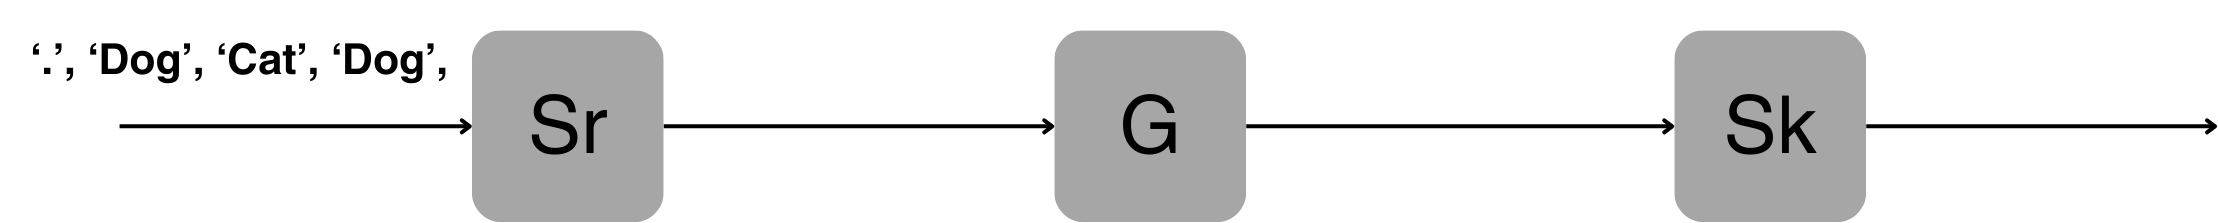
\includegraphics[width=1\textwidth]{DP104.png}
    \caption[{[Lib]} Counting words inital state]{Initial state of the Dynamic Pipeline with the input prepared}
    \label{fig:DP104}
\end{figure}

The first word, 'Dog', will go through the Sr and turn it into a tuple (Dog, 0).
This reaches the generator and generates the first filter, since it is an initial data (counter to 0).
The Sr continues to process the input while following the process.

\begin{figure}[H]
    \centering
    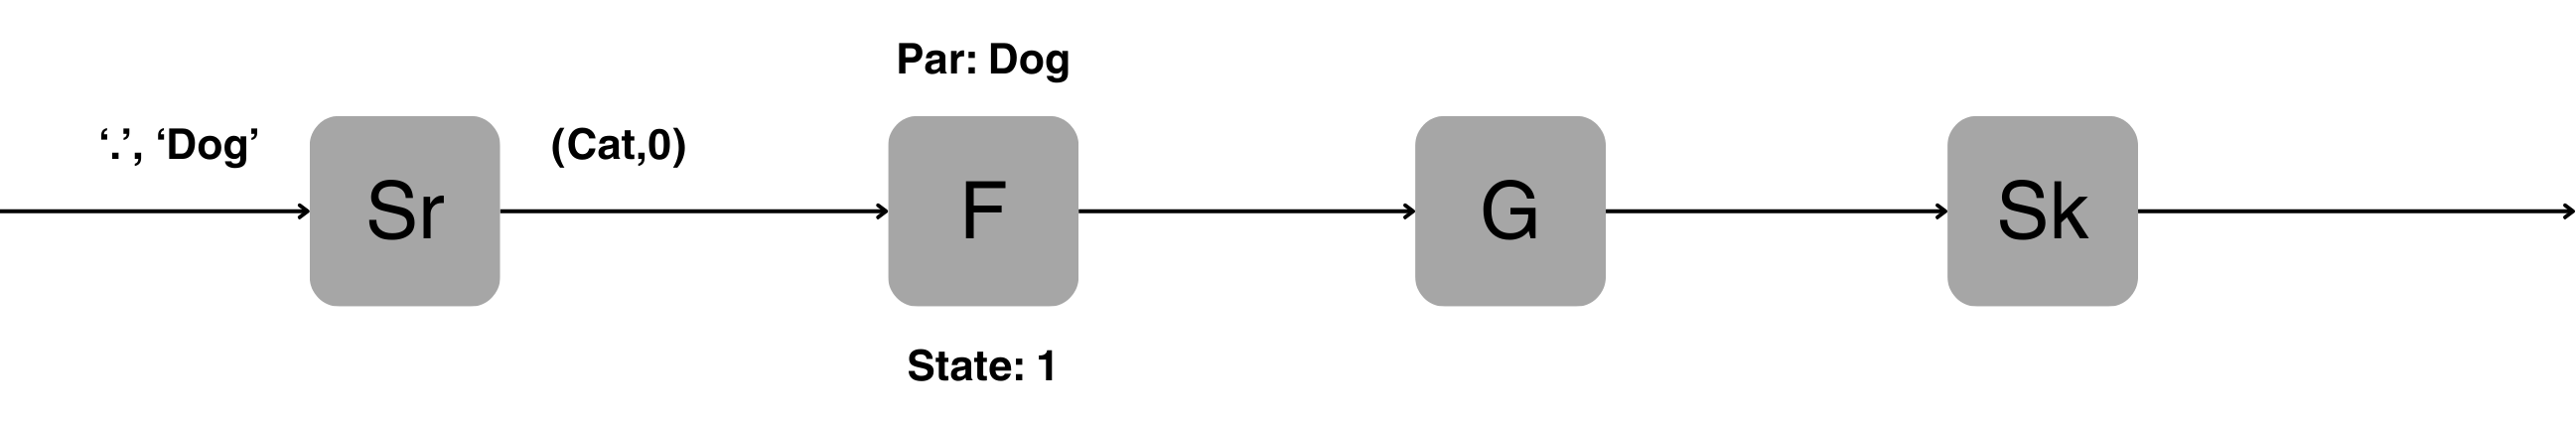
\includegraphics[width=1\textwidth]{DP105.png}
    \caption[{[Lib]} Counting words state 1]{State of Dynamic Pipeline after consuming some words}
    \label{fig:DP105}
\end{figure}

If we continue executing until just after the Sr processes the '.', this is the state of our pipeline:

\begin{figure}[H]
    \centering
    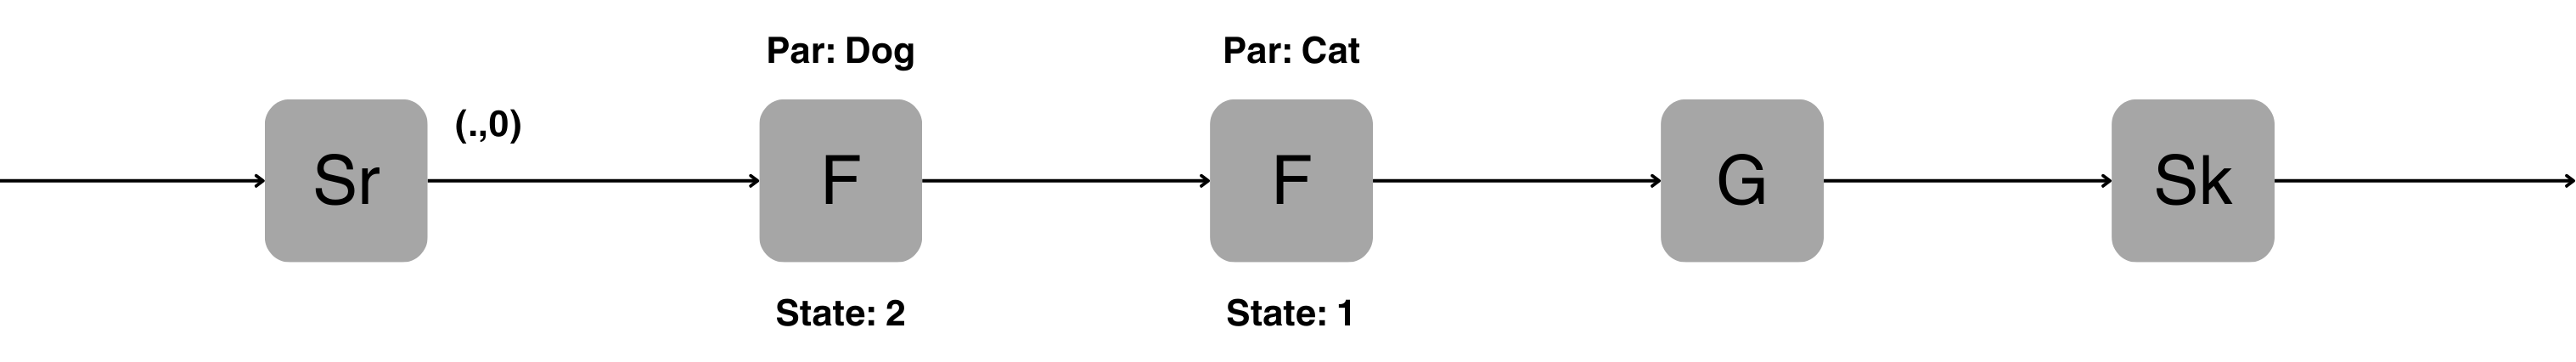
\includegraphics[width=1\textwidth]{DP106.png}
    \caption[{[Lib]} Counting words state 2]{State of Dynamic Pipeline before the '.' is processed by filters}
    \label{fig:DP106}
\end{figure}

When the '.' starts to be processed by F's, they with start to throw partial results.
This is the view of the pipeline before the second F starts to process the '.'.

\begin{figure}[H]
    \centering
    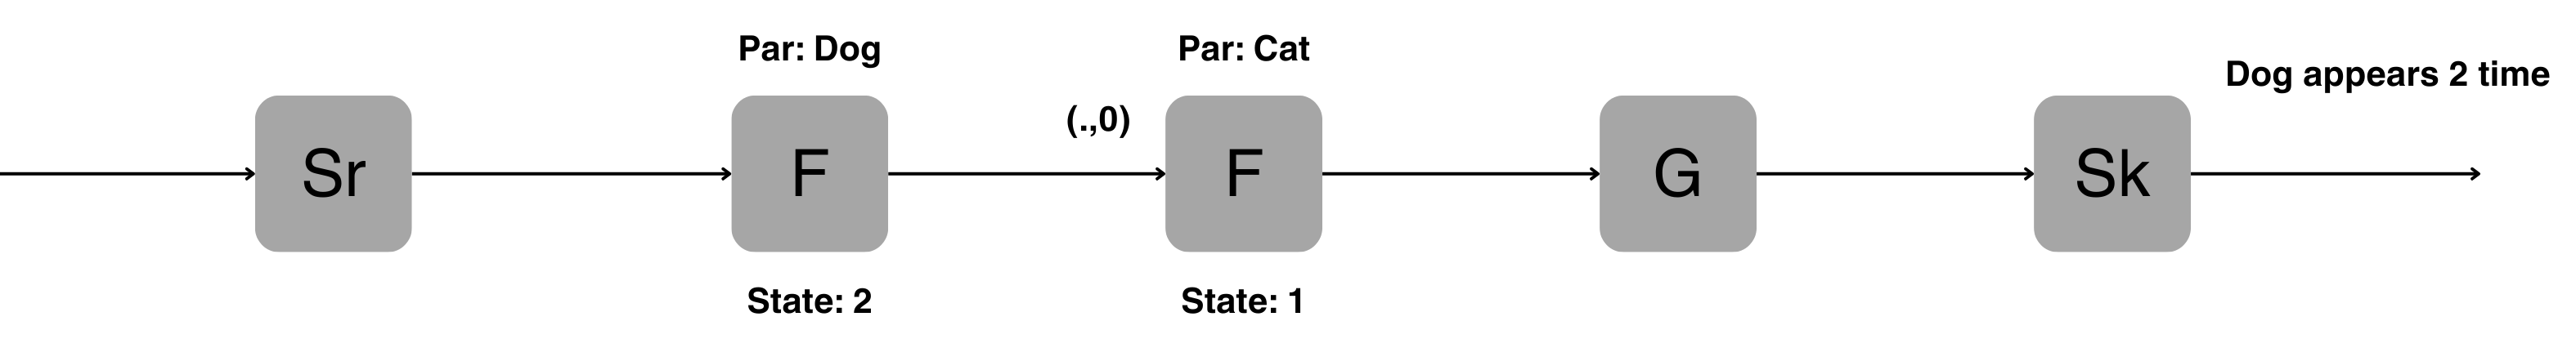
\includegraphics[width=1\textwidth]{DP107.png}
    \caption[{[Lib]} Counting words state 3]{State of Dynamic Pipeline before the the second filter processes the '.'}
    \label{fig:DP107}
\end{figure}

And this is the final state after the whole execution:

\begin{figure}[H]
    \centering
    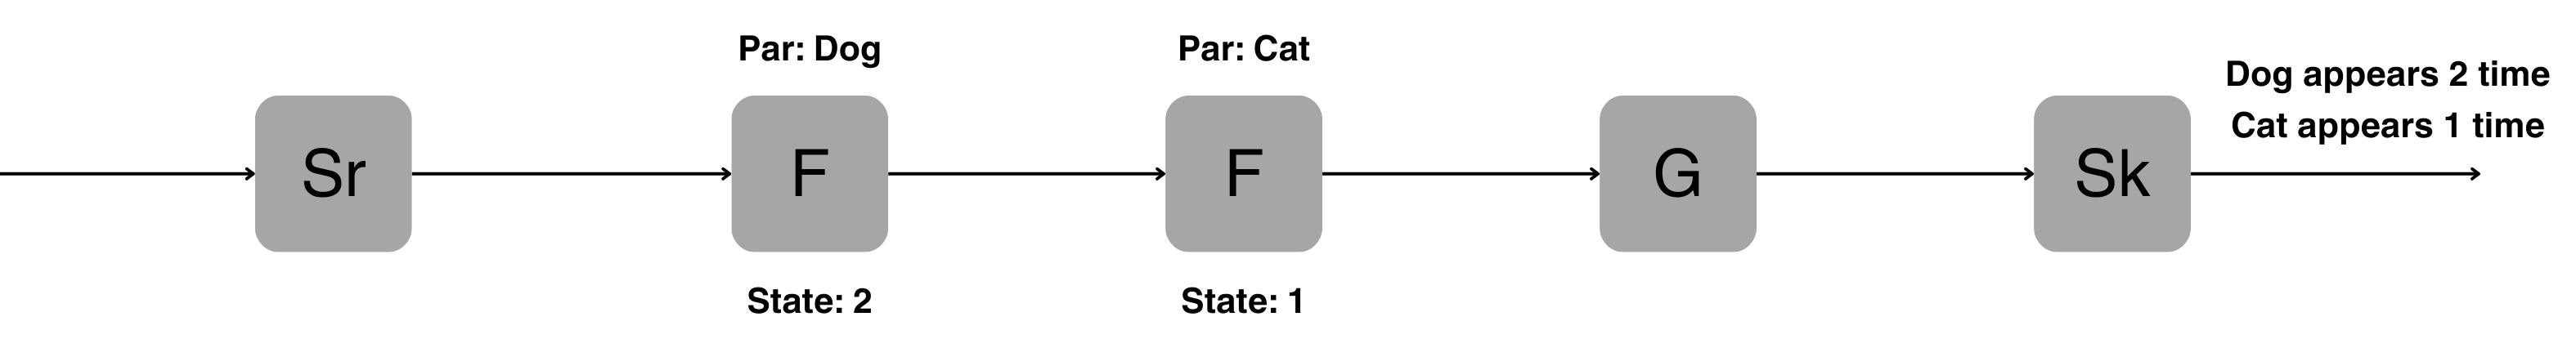
\includegraphics[width=1\textwidth]{DP108.png}
    \caption[{[Lib]} Counting words final state]{Final state of the Dynamic Pipeline}
    \label{fig:DP108}
\end{figure}

\subsection{Algorithm Implementation}
Now we have all the components necessary to use the library in a real case: We understand how a Dynamic Pipeline works, we know how to implement it using the Haskell library and we have defined an algorithm for a specific problem. Now we just have to apply everything.
\subsubsection*{Type definition}
Let's start by defining our Dynamic Pipeline structure in Haskell:

\begin{figure}[H]
    %\centering
    \begin{tabular}{c}
        \begin{lstlisting}
type Word = String
type Pair = (Word,Int)
type filtStat = Int
type filtPar = Pair
type DPExample = Source (Channel (Pair :<+> Eof)) 
                :=> Generator (Channel (Pair :<+> Eof)) 
                :=> Sink
        \end{lstlisting}
    \end{tabular}
    \caption[{[Code]} Implementation 1]{Type definition of the Dynamic Pipeline}
    \label{fig:HC16}
\end{figure}

I've also defined some additional types for the tuples and for the state and parameters of the F filter, for simplicity.

\subsubsection*{Source}
As we determined earlier, to define the source we only have to implement 1 function (which we have called fillChannels)

\begin{figure}[H]
    \begin{tabular}{c}
        \begin{lstlisting}
input :: [Word]
input = ["Dog","Cat","Dog","."]

source' :: Stage (WriteChannel Pair -> DP s ())
source' = withSource @DPExample fillChannels

fillChannels :: WriteChannel Pair
             -> DP st ()
fillChannels wp = unfoldT input wp (*\$*) \w -> (w,0)
        \end{lstlisting}
    \end{tabular}
    \caption[{[Code]} Implementation 2]{Implementation of fillChannels function}
    \label{fig:HC17}
\end{figure}

We can observe how the fillChannels function uses the unfoldT function provided by the library to read an array and pass it through a write channel.
We also use an anonymous function to transform the words into tuples.

\subsubsection*{Sink}
For this stage, we need to implement the readChannels function:

\begin{figure}[H]
    %\centering
    \begin{tabular}{c}
        \begin{lstlisting}
sink' :: Stage (ReadChannel Pair -> DP s ())
sink' = withSink @DPExample readChannels

readChannels ::ReadChannel Pair -> DP st ()
readChannels rp = foldM_ rp printResults

printResults :: Pair -> DP st ()
printResults (".",_) = print "**********************"
printResults (w,n) = print $ w ++ " " ++ show n

        \end{lstlisting}
    \end{tabular}
    \caption[{[Code]} Implementation 3]{Implementation of readChannels function}
    \label{fig:HC18}
\end{figure}

In this case, we use the unique function provided by the library: foldM function.
It reads a channel and do a function, in this case, print the results.

\subsubsection*{Filter}
For the F we need to implement all the actors.
As we have only one actor, we will only implement one function.

\begin{figure}[H]
    %\centering
    \begin{tabular}{c}
        \begin{lstlisting}
filterTemp :: Filter DPExample filtStat filtPar s 
filterTemp = mkFilter actor1

actor1 :: filtPar
        -> ReadChannel Pair
        -> WriteChannel Pair
        -> StateT filtStat (DP s) ()
actor1 (par,_) rp wp =
  foldM_ rp (*\$*) \(inp,y) -> 
    if inp == "." 
    then get >>= \x -> push (par,x) wp >> push (".",0) wp
    else    if inp == par
            then modify (+1)
            else push (inp,y) wp
        \end{lstlisting}
    \end{tabular}
    \caption[{[Code]} Implementation 4]{Implementation of actor}
    \label{fig:HC19}
\end{figure}

As we defined before, it treats each element with the foldM function following the chain of if's: first if it's a period, where it would pass the result and the period.
Otherwise, it would update the state with the modify function or simply let the word pass through.

\subsubsection*{Generator}
Finally, we have to implement the G stage:

\begin{figure}[H]
    %\centering
    \begin{tabular}{c}
        \begin{lstlisting}
generator' :: GeneratorStage DPExample filtStat filtPar s
generator' = let gen = withGenerator @DPExample genAction
            in  mkGenerator gen filterTemp

genAction :: Filter DPExample filtStat filtPar s
          -> ReadChannel Pair
          -> WriteChannel Pair
          -> DP s ()
genAction filter rp wp =
  let unfoldFilter = 
  mkUnfoldFilter create (moveOn wp) filter iniFilter rp HNil
  in void $ unfoldF unfoldFilter

create :: Pair-> Bool
create (".",_) = False
create (_,0) = True
create _ = False

moveOn :: WriteChannel Pair -> Pair -> DP s ()
moveOn c (".",_) = push (".",0) c
moveOn _ (_,0) = return ()
moveOn c a = push a c

iniFilter :: Pair -> filtStat
iniFilter _ = 1
        \end{lstlisting}
    \end{tabular}
    \caption[{[Code]} Implementation 5]{Implementation of generator}
    \label{fig:HC20}
\end{figure}

This stage involves defining the most functions, although the mkUnfoldFilter constructor aids significantly in implementation.
The three generator functionalities must be implemented: determining under which conditions to generate a filter, initializing a filter, and deciding which elements to pass through.
To achieve this, three functions have been defined: create, iniFilter, and moveOn, which handle the aforementioned functionalities, respectively.
The \textit{create} function takes an element of the input channel type and returns a boolean value indicating whether or not to generate a filter. \\
Similarly, the \textit{iniFilter} function takes an element of the input channel type and returns an element of the filter state type. \\
Finally, the \textit{moveOn} function receives both the write channel and an element of the channel type and decides whether to push the element or do nothing (effectively discarding the element). 

\subsection{Conclusions}
In this section, we have seen the entire process for implementing a simple problem like counting words.
To test its effectiveness, some tests have been carried out. This is a tested input:

\begin{center}
input = ["dog", "cat",".","dog","dog","dog",".","bird","cat","."]
\end{center}
And this has been the result obtained:

\begin{center}
"dog 1" \\
"cat 1" \\
"**********************" \\
"dog 4" \\
"cat 1" \\
"**********************" \\
"dog 4" \\
"cat 2" \\
"bird 1" \\
"**********************" \\
\end{center}

Therefore, we can conclude that the implementation has been developed successfully
\section{Improving the library}
After working with the library, I have been able to identify different shortcomings and lack of functionalities for a more diverse and easier use of the library.
In this section, I will detail and comment on different improvements that I have added to the library.

\subsection{New features}
\subsubsection*{unfoldFilebyChars}

When I was working with the library, the first thing I missed was having more tools to work with the input.
The library has the functions unfoldM, unfoldFile, and unfoldT to handle general monadic inputs, files, and lists, respectively.
The problem is that the unfoldFile function only reads files line by line, since that's how it was useful for Juan Pablo's problem.
That's why I decided to create this function to be able to read character by character for letters of the alphabet.
In this way, the channel is fed with characters and it can be, for example, the F or the G that are responsible for finding the desired format.

\begin{figure}[H]
    %\centering
    \begin{tabular}{c}
        \begin{lstlisting}
unfoldFilebyChars :: FilePath 
                    -> WriteChannel a 
                    -> (ByteString -> a) 
                    -> DP s ()
unfoldFilebyChars file writeChannel fn =
  liftIO $ R.withFile file ReadMode $ \h -> 
        unfoldM (hGetchar h) fn (H.hIsEOF h) writeChannel

hGetchar :: Handle -> IO ByteString
hGetchar h = do
    c <- hGet h 1
    if c == "" || c == "." || "a" <= c && c <= "z" 
    then return c 
    else hGetchar h
        \end{lstlisting}
    \end{tabular}
    \caption[{[Code]} unfoldFilebyChars definition]{unfoldFilebyChars function}
    \label{fig:HC21}
\end{figure}

An example usage of the function is as follows:

\begin{figure}[H]
    %\centering
    \begin{tabular}{c}
        \begin{lstlisting}
-- Write Channel (wc) Type = String
unfoldFilebyChars "example.txt" wc decodeUtf8	
        \end{lstlisting}
    \end{tabular}
    \caption[{[Code]} unfoldFilebyChars example]{unfoldFilebyChars function usage}
    \label{fig:HC21b}
\end{figure}

\subsubsection*{unfoldFilebyWords}
Similar to the previous function, this function feeds a channel from a file by reading the words.
It separates the input by the blank space character ' ' similar to the getContents function in Haskell. \\

This improvement is quite significant, offering considerably more flexibility than the existing function.
The ability to retrieve content item by item rather than the entire row facilitates simpler input processing.
\begin{figure}[H]
    %\centering
    \begin{tabular}{c}
        \begin{lstlisting}
unfoldFilebyWords :: FilePath 
            -> WriteChannel a --Write Channel to feed
            -> (ByteString -> a) --Map ByteString to type a
            -> DP s ()
unfoldFilebyWords file writeChannel fn = 
  liftIO $ R.withFile file ReadMode $ \h -> 
        unfoldM (hGetWord h) fn (H.hIsEOF h) writeChannel

hGetWord :: Handle 
        -> IO ByteString
hGetWord h = hGetWordRec h B.empty

hGetWordRec :: Handle 
            -> ByteString 
            -> IO ByteString
hGetWordRec h r = do
    c <- B.hGet h 1
    if c == "" || c == " " || c == "\n" then return r
    else do
        cs <- hGetWordRec h (B.append r c)
        return cs
        \end{lstlisting}
    \end{tabular}
    \caption[{[Code]} unfoldFilebyWords definition]{unfoldFilebyWords function}
    \label{fig:HC22}
\end{figure}

An example usage of the function is as follows:

\begin{figure}[H]
    %\centering
    \begin{tabular}{c}
        \begin{lstlisting}
-- Write Channel (wc) Type = String
unfoldFilebyWords "example.txt" wc decodeUtf8	
        \end{lstlisting}
    \end{tabular}
    \caption[{[Code]} unfoldFilebyWords example]{unfoldFilebyWords function usage}
    \label{fig:HC22b}
\end{figure}

\subsubsection*{pushState}
While not essential for the library's core functionality, this function aims to streamline the implementation process.
Often, retrieving and passing the filter state through a channel is required.
This function simplifies this task, enhancing ease of use.
Additionally, an optional function 'f' can be provided to convert the filter state type to the channel type.

\begin{figure}[H]
    %\centering
    \begin{tabular}{c}
        \begin{lstlisting}
pushState :: WriteChannel a --Write Channel to feed
            -> (b -> a) --Map state type to channel type
            -> StateT b (DP s) ()
pushState wp f = get >>= flip push wp . f
        \end{lstlisting}
    \end{tabular}
    \caption[{[Code]} pushState definition]{pushState function}
    \label{fig:HC23}
\end{figure}
An example usage of the function is as follows:

\begin{figure}[H]
    %\centering
    \begin{tabular}{c}
        \begin{lstlisting}
-- filtStat Type = Int
-- Write Channel (wc) Type = String
pushState wc show
        \end{lstlisting}
    \end{tabular}
    \caption[{[Code]} pushState example]{pushState function usage}
    \label{fig:HC23b}
\end{figure}

\subsubsection*{foldFile}
Another major problem I encountered was that the library also had almost no functions for handling output in a simple way.
The library has the foldM function, which is a very generic function for consuming a channel.
That's why I decided to add this function, which consumes a channel and writes it to an output file.
At the beginning of writing, the file is created if it does not exist, or the file is cleaned if it already existed. \\

This new functionality is highly desirable, especially when dealing with large inputs or performing analyses.
It allows us to gather all results in a convenient format, enabling more efficient processing and reading.

\begin{figure}[H]
    %\centering
    \begin{tabular}{c}
        \begin{lstlisting}
foldFile:: MonadIO m 
        => FilePath     --Path of file 
        -> (a -> Text)  -- Map WriteChannel type a to Text
        -> ReadChannel a --ReadChannel to read
        -> m ()
foldFile file f rc = do
  writeFileText file T.empty
  foldM_ rc (R.appendFileText file . f)
        \end{lstlisting}
    \end{tabular}
    \caption[{[Code]} foldFile definition]{foldFile function}
    \label{fig:HC24}
\end{figure}

An example usage of the function is as follows:

\begin{figure}[H]
    %\centering
    \begin{tabular}{c}
        \begin{lstlisting}
-- Read Channel (rc) Type = String
foldFile "example.txt" toText rc	
        \end{lstlisting}
    \end{tabular}
    \caption[{[Code]} foldFile example]{foldFile function usage}
    \label{fig:HC24b}
\end{figure}

\subsection{Updating the library to a newer version of GHC}
In this section, we will update the library to be compatible with newer versions of GHC, the Haskell compiler.
Currently, the library supports GHC version 8.10.3 and will be updated to support version 9.0.2.
This specific version was chosen as it's the latest supported by all libraries utilized by Dynamic Pipeline.
Particularly, the HList library introduces compatibility issues with newer GHC versions.
Updating the libraries would be necessary to leverage newer compiler versions.\\

The library consists of four source files: Flow.hs, Stage.hs, Channel.hs, and DynamicPipeline.hs.
DynamicPipeline is the main file and encompasses the other three, hence the need to update all of them.\\

This is the first error encountered when trying to compile DynamicPipeline.hs with the new GHC version:

\begin{figure}[H]
    %\centering
    \begin{tabular}{c}
        \begin{lstlisting}[escapeinside={(*}{*)}, language=bash]
DynamicPipeline/Stage.hs:515:9: (*\textcolor{red}{error:}*)
    Couldnt match type: DP st0 a
        with: forall (st :: k). DP st a
    Expected: (forall (st :: k). DP st a) -> IO a
        Actual: DP st0 a -> IO a
    In the expression: runStage
    In an equation for 'runDP': runDP = runStage
    Relevant bindings include
        runDP :: (forall (st :: k). DP st a) -> IO a
            (bound at DynamicPipeline/Stage.hs:515:1)
    (*\textcolor{blue}{|}*)
(*\textcolor{blue}{515}*)  (*\textcolor{blue}{|}*) runDP = (*\textcolor{red}{runStage}*)
    (*\textcolor{blue}{|}*)
        \end{lstlisting}
    \end{tabular}
    \caption[{[Lib] First console output} unfoldFilebyChars definition]{Console output after compiling DynamicPipeline.hs with GHC 9.0.2}
    \label{fig:HC25}
\end{figure}

And here is the code for the function that generates the error:

\begin{figure}[H]
    %\centering
    \begin{tabular}{c}
        \begin{lstlisting}
runDP :: (forall st. DP st a) -> IO a
runDP = runStage
        \end{lstlisting}
    \end{tabular}
    \caption[{[Code]} runDP error]{Piece of code generating the error}
    \label{fig:HC26}
\end{figure}
What we can gather from this error is that there's a type inference issue with the runDP function in the Stage.hs file.
Based on the observation, it seems that newer GHC versions are stricter with polymorphic types.
Delving into the GHC documentation, the first relevant information we find is that the initial GHC 9 release (9.0.1) introduced the following feature: \cite*[][Point 2.1.2.1]{} \\

\textit{"Record field selectors are now given type signatures that preserve the user-written order of quantified type variables.
Moreover, field selector type signatures no longer make inferred type variables available for explicit type application."}  \\

If we apply the new restrictions detailed in the release notes, our code would now look like this:

\begin{figure}[H]
    %\centering
    \begin{tabular}{c}
        \begin{lstlisting}
runDP :: forall {k} (st :: k) a. DP st a -> IO a
runDP = runStage
        \end{lstlisting}
    \end{tabular}
    \caption[{[Code]} New runDP definition]{New version of the code}
    \label{fig:HC27}
\end{figure}

As we can see now, we need to explicitly state that the type of st is any.
With this change, the compilation error no longer appears, so this part is now resolved.
However, when compiling again, there are still some errors to address.
There is a large output in the console, and here is some of the relevant information:

\begin{figure}[H]
    %\centering
    \begin{tabular}{c}
        \begin{lstlisting}[escapeinside={(*}{*)}, language=bash]
            .
            .
            .
DynamicPipeline/Stage.hs:408:29: (*\textcolor{red}{error:}*)
Couldnt match type 'b0'
    with MonadState filtStat monadicAction =>
    Stage (WithFilter dpDef filterParam monadicAction)
Expected: 
    Actor dpDef filtStat filterParam monadicAction
    -> b0
Actual: 
    Actor dpDef filtStat filterParam monadicAction
    -> MonadState filtStat monadicAction =>
    Stage (WithFilter dpDef filterParam monadicAction)
            .
            .
            .
    (*\textcolor{blue}{|}*)
(*\textcolor{blue}{408}*)  (*\textcolor{blue}{|}*) runActor = hUncurry . run . (*\textcolor{red}{unActor}*)
    (*\textcolor{blue}{|}*)
        \end{lstlisting}
    \end{tabular}
    \caption[{[Lib] Second console output}]{Second console output after compiling DynamicPipeline.hs with GHC 9.0.2}
    \label{fig:HC28}
\end{figure}

Similar to the previous error, here we also have a type inference problem.
Once again, the GHC update has made it stricter, causing us to have to modify the code to fix it.

If we see, the funcion unActor is the problem, so here is the code of the definition:

\begin{figure}[H]
    %\centering
    \begin{tabular}{c}
        \begin{lstlisting}
newtype Actor dpDef filtStat 
                filterParam monadicAction =
  Actor {unActor :: 
    MonadState filtStat monadicAction => 
  Stage (WithFilter dpDefinition filterParam monadicAction)}
        \end{lstlisting}
    \end{tabular}
    \caption[{[Code]} unActor error]{Piece of code generating the error}
    \label{fig:HC29}
\end{figure}

Starting with GHC version 9.0.1, it was added that new type definitions had to be explicit, so the way we have it here can no longer be used.
Therefore, we must leave the code like this:
\begin{figure}[H]
    %\centering
    \begin{tabular}{c}
        \begin{lstlisting}
newtype Actor dpDef filtStat 
                filterParam monadicAction =
Actor {unActor ::
  Stage (WithFilter dpDef filterParam monadicAction)}
        \end{lstlisting}
    \end{tabular}
    \caption[{[Code]} New unActor]{New version of the code}
    \label{fig:HC30}
\end{figure}
With these changes, we have now been able to compile the library with GHC 9.0.2.

\section{Chapter summary}
In this section, we have been able to improve the Haskell Dynamic Pipeline library.
We have added new features to make it easier to implement new algorithms, and we have also updated the library to support GHC 9.0.2.
With these advances, I aim to ensure that the library remains usable and does not become outdated.
At the end of the work \ref{experiments}, an experimental test will be carried out to verify if an improvement in the performance of the library has also been obtained.


\chapter{Improving the IEBT algorithm} \label{IEBT}
This is the second part of my work, where I will try to find and argue for different improvements for the implementation of the algorithm for incremental enumeration of Bitriagles (IEBT).
This implementation developed by Juan Pablo uses the Dynamic Pipeline library with which I have been working.
The entire first part of my work has been necessary to fully understand the operation of both the dynamic pipeline paradigm itself and the operation of the Haskell library.

\section{Introduction}
A brief introduction to understand the basic concepts is provided here.
For a more detailed explanation, refer to Royo-Sales et al. \cite[][See chapter 6]{royo_sales_algorithm_2021} \\
The IEBT algorithm involves finding bitriangles in a bipartite graph.
\begin{figure}[H]
  \centering
  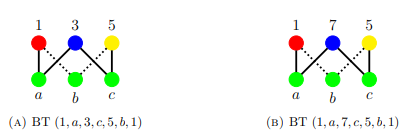
\includegraphics[width=1\textwidth]{JP1.png}
  \caption[{[IEBT] BiTriangle}]{Bitriangle structure, taken from \cite{royo_sales_algorithm_2021}}
  \label{fig:JP1}
\end{figure}
To achieve this, it groups vertices into different structures until it reaches a structure that forms many bitriangles. \\
The process is as follows: initially, all the edges of the graph are processed, and the generator creates a filter for each edge it receives, initializing it with that edge.
The filters process the edges and check the vertices to find a match with their parameter.
If a match is found, it consumes the edge and adds it to its state, thus forming the Aggregated Wedges.
\begin{figure}[H]
  \centering
  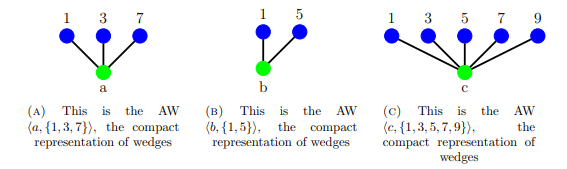
\includegraphics[width=1\textwidth]{JP2.png}
  \caption[{[IEBT] Aggregated Wedges}]{Aggregated Wedges strucute, taken from \cite{royo_sales_algorithm_2021}}
  \label{fig:JP2}
\end{figure}
Once all the edges have been processed, the filters send the AWs generated by the pipeline so that they can be combined to form the Aggregated Double-Wedges.

\begin{figure}[H]
  \centering
  \includegraphics[width=1\textwidth]{JP3.png}
  \caption[{[IEBT] Aggregated Doble Wedges}]{Aggregated Doble Wedges structure, taken from \cite{royo_sales_algorithm_2021}}
  \label{fig:JP3}
\end{figure}

Once the filters have these structures, queries can be sent through the pipeline to obtain the bitriangles.
\section{Improving structures}
The first topic I wanted to address was the data types used to store the different sets.
The algorithm needs to store different vertex structures for later matching.
These are the different definitions found in the code:

\begin{figure}[H]
    %\centering
    \begin{tabular}{c}
        \begin{lstlisting}[escapeinside={(*}{*)}]
type LowerVertex = Int
type UpperVertex = Int
type Edge = (UpperVertex, LowerVertex)

data Command = ByVertex IntSet
            | ByEdge (Set Edge)
            | Count
            | AllBT
            | NoCommand
            | End
        deriving (Show, Read)

data W = W
  { _wLowerVertex :: LowerVertex
  , _wWedges      :: IntSet
  }
  deriving Show

data Triplet = Triplet Int Int Int
data Pair = Pair Int Int

type UT = (IntSet, IntSet, IntSet)

data DW = DW
  { _dwLower :: Pair
  , _dwUpper :: UT
  }

newtype DWTT = DWTT [DW]
  deriving newtype (Semigroup, Monoid)

data BT = BT
  { _btLower :: Triplet
  , _btUpper :: UT
  }

newtype BTTT = BTTT [BT]
  deriving newtype (Semigroup, Monoid)

data BTResult = RBT Q (Int, Int, Int, Int, Int, Int, Int)
              | RC  Q Int

data FilterState = Adj W
                 | DoubleWedges DWTT
                 | BiTriangles BTTT
        \end{lstlisting}
    \end{tabular}
    \caption[{[IEBT] Type and data definitions}]{Type and data definitions of IEBT implementation}
    \label{fig:HC40}
\end{figure}


We can see how it represents vertices with integers Int and edges as tuples of integers (Int, Int).
The most important thing to analyze are the set representations, as their impact on the performance of the algorithm is crucial.
It uses the IntSet structure to represent sets of vertices and also a tuple of 3 IntSets (IntSet, IntSet, IntSet) to represent the set of upper vertex of the Aggregated Doble Wedge and Aggregated Bitriangles. \cite[][Page52]{royo_sales_algorithm_2021}
Also taking into account the use of lists to represent the set of Aggregated Double Wedges and Aggregated Bitriangles. \\

We will be analizing structure by structure trying to find if the structure used is the most efficient.
\subsection{Set of vertices representation}
The IntSet structure belongs to the Haskell IntSet library \cite{noauthor_dataintset_nodate}, which represents an ordered set of Ints.
This structure is very efficient because it takes advantage of the range limit of Ints to limit many operations to a cost of O(min(n,W)), where n is the number of elements and W is the number of bits in the Int representation (32 or 64).
Additionally, this structure is based on big-endian patricia trees, which have very good performance for set intersection and union operations.

\subsubsection*{Wedges representation}
If we review the first structure that use IntSet, we can see that filters can have three types of states, one of which is the Wedge, which uses this structure.
To understand how this structure is used (and therefore whether or not it can be improved), we need to know what computations are performed with it.
Observing the code, we can see that only two of the four actors that each filter has deal with W: actor1 and actor2.\\
On the part of actor1, for each input edge, a condition is checked and if it is affirmative, a vertex is attached to the IntSet set.
Therefore, in the worst case, insertions will have to be made and each insertion has a cost of O(n,W), and assuming a sufficiently large n, we are left with O(W) = O(1). \\
On the other hand, actor2 performs difference and intersection operations with the IntSets.
These operations with this library have a linear cost with respect to the size of the sets O(n + m). \\

Looking at these costs, we can conclude that a very efficient structure seems to be used.
We could also use a Hash-type structure, such as a HashSet, to improve the performance of insertions.
Reviewing the Haskell libraries, we find the HashSet structure.
Despite being useful, the documentation itself warns us that for Int sets, the IntSet library is more efficient.
Therefore, for Wedges, IntSets are the best structure.

\subsubsection*{Doble Wedges and Agregated Bitriangles representation}
Next, we should focus on the definition of the UT type, which is formed by a tuple of 3 IntSets.
If we review the entire code for functions that use it, we find a similar scenario to the previous one.
In general, insertion operations are performed on the sets, and the choice of IntSet is correct. \\

On the other hand, the other important operation that is performed is to check if a vertex belongs to any of the 3 sets.
To do this, it checks each of the 3 sets, so it might be possible to optimize this process a bit.
Despite this, the best option that could be done is to try to join the 3 sets so that you only have to search in a larger one, asymptotically reducing the cost by 3.
The problem is that we would have to find another way to represent the 3 sets, such as with indexes using a dictionary.
For this reason, I have considered that the cost of carrying this structure and other operations that are done on it increases greatly for the improvement we obtain, so I do not see any possible improvement in this regard. \\

Therefore, the choice of this structure is the correct one to represent the UTs.

\subsection{Set of edges representation}
The next thing to observe is the representation of edge sets.
As such, the entire algorithm does not store any edge sets, as it plays with the structure of the different types to infer the edges.
There is only one thing for which edges are used: the final Queries. \\

At this stage, a set of edges can be passed to find bitriangles that contain it, and for this, it uses the Set to store them.
In this case, the only operation that is done is to check whether an edge is inside or not.
Therefore, I have determined that a possible improvement could be to change the Set, which has a search cost of O(log n), to one that has better performance, such as the HashSet.
The HashSet has a cost, in the general case, of constant O(1). \\

Therefore, I have changed the Set structure to HashSet to look for a performance improvement.
At the end of the work \ref{experiments}, an experimental test will be carried out to verify whether there is an improvement or not.

\section{Chapter Summary}
In this chapter, we have been analyzing the implementation of the IEBT algorithm to try to find an improvement. \\
Despite the fact that the beginning of this work arose with the belief that it could be improved, I have not been able to find a possible significant improvement for the implementation of the IEBT algorithm.

\chapter{Experiments} \label{experiments}
In this chapter, we will carry out some experiments to test the improvements made in chapters \ref{IDPL} and \ref{IEBT}.
For the execution of the programs, I will be using an Asus VivoBook 15 X540UB laptop. These are the technical specifications of the laptop:
\begin{itemize}
  \item \textbf{Processor:}  Intel Core i5-8250U CPU @ 1.60GHz
  \item \textbf{Memory}  8GB RAM
  \item \textbf{Graphics adapter:} Intel UHD Graphics 620
  \item \textbf{Storage:} 256 SSD
  \item \textbf{Operating System:} Windows 10 Home 64-bit
\end{itemize}
To ensure better results, they will all be executed with the laptop running only that process.
In all experiments, only the execution time will be evaluated.
Memory usage would remain to be checked to complete the evaluation.\\
All the experiments and results can be found in the 'Experiments' folder on Github. \cite{forner_gomez_source_nodate}

\section{Testing Library}
The main improvement that can affect the performance of the library is the update of GHC.
To test this, we will use the toy problem developed during this work.
We will modify it a bit by counting characters instead of words, in order to be able to test larger inputs more efficiently.
We will limit the characters to those of the alphabet (plus the dot for the incremental character) thus ensuring that there will be at most 26 filters.
\subsection*{Input}
The text of Don Quixote has been used as input, which has been modified to convert or eliminate any unwanted characters.
To do this function, a python script has been used that also allows generating inputs of a specific size.
Inputs of powers of 10 will be used, from 10 to 100000.

\subsection*{Results}
These are the results of running 10 times for each size and taking the mean and standard deviation.

\begin{table}[H]
    \begin{adjustwidth}{-1in}{-1in} % Adjust margins by -1 inch on both sides
    \centering
    \begin{tabular}{|c|c|c|c|c|c|c|c|c|c|c|c|c|}
    \hline
    size & mean (s)& std (s) \\
    \hline
    10 & 0.029994 & 0.012285 \\
    100 & 0.100318 & 0.008902 \\
    1000 & 0.971935 & 0.097618 \\
    10000 & 11.619426 & 0.835211 \\
    100000 & 231.629199 & 1.330213 \\
    \hline
    \end{tabular}
    \caption[{[Exp] Table results GHC 8.10.3}]{Results 10 executions using GHC 8.10.3}
    \label{results1}
    \end{adjustwidth}
\end{table}

\begin{table}[H]
    \begin{adjustwidth}{-1in}{-1in} % Adjust margins by -1 inch on both sides
    \centering
    \begin{tabular}{|c|c|c|c|c|c|c|c|c|c|c|c|c|}
    \hline
    size & mean (s)& std (s) \\
    \hline
    10 & 0.005374 & 0.001071 \\
    100 & 0.091677 & 0.004923 \\
    1000 & 0.881183 & 0.067268 \\
    10000 & 9.786606 & 0.606498 \\
    100000 & 159.005325 & 1.553883 \\
    \hline
    \end{tabular}
    \caption[{[Exp] Table results GHC 9.0.2}]{Results 10 executions using GHC 9.0.2}
    \label{results2}
    \end{adjustwidth}
\end{table}

\begin{figure}[H]
    \centering
    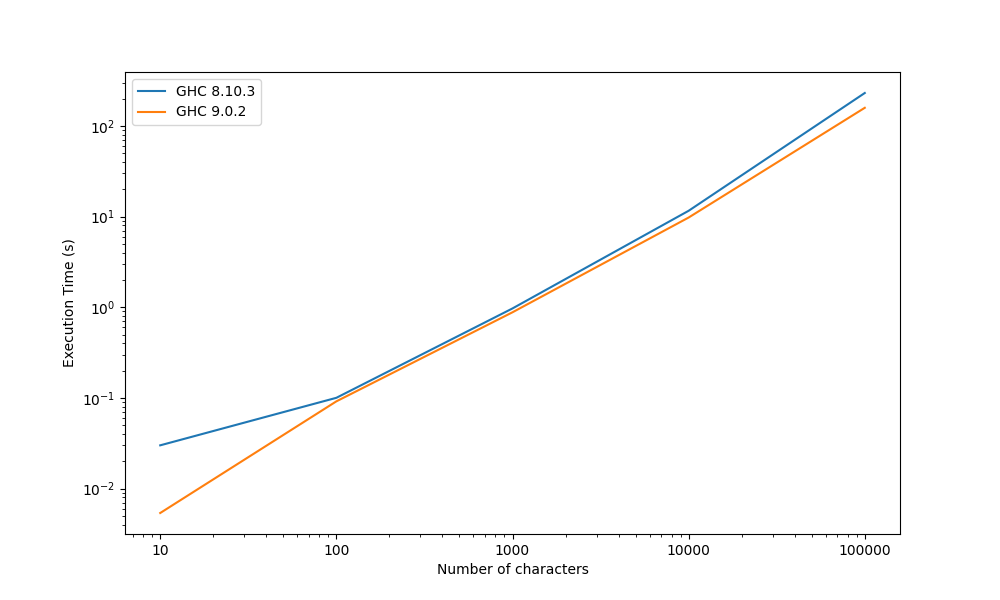
\includegraphics[width=1\textwidth]{ExecutionPlot.png}
    \caption[{[Exp] Plot GHC 8.10.3 vs 9.0.2}]{Plot of execution mean time vs input size for GHC 8.10.3 and GHC 9.0.2}
    \label{fig:results3}
\end{figure}

\subsection*{Discussion}
As we can observe, there seems to be a slight improvement with GHC 9.02 compared to GHC 8.10.3, even in some more noticeable cases. \\

We can see how for much smaller inputs the new version tends to obtain better results, which could be due to better management when creating the filters.
In smaller inputs, the task that is done the most is generating filters, because with larger inputs there comes a point where the 26 filters have already been generated (one for each letter) and no more are generated.
Perhaps better memory management by the compiler is causing this improvement. \\
On the other hand, we can observe how in the central part the two have a similar performance, although the new version is still slightly better. \\
Finally, we can see how with larger inputs the new version again has better performance, this time more noticeable. \\

In summary, although it seems that with the update to GHC 9.0.2 there is an improvement, we do not obtain very clear results.
Other factors such as memory would have to be checked to conclude with a result.

\section{Testing IEBT}
In this experiment, we will test the change of structure from Set to HashSet implemented in the IEBT algorithm.

\subsection*{Input}
For this experiment, we will be using a bipartite graph of 3000 edges and we will make queries from size 1000 edges to 3000.

\subsection*{Results}
This is the result of running each size 5 times and obtaining the mean and standard deviation.

\begin{table}[H]
    \begin{adjustwidth}{-1in}{-1in}
    \centering
    \begin{tabular}{|c|c|c|c|c|c|c|c|c|c|c|c|c|}
    \hline
    size & mean (s)& std (s) \\
    \hline
    1000 & 5.570314 & 0.560374 \\
    1500 & 7.731554 & 1.032222 \\
    2000 & 8.778615 & 1.534666 \\
    2500 & 9.506494 & 0.579319 \\
    3000 & 12.134800 & 2.795664 \\
    \hline
    \end{tabular}
    \caption[{[Exp] Table results Set structure}]{Results 5 executions using Set structure}
    \label{results4}
    \end{adjustwidth}
\end{table}

\begin{table}[H]
    \begin{adjustwidth}{-1in}{-1in} % Adjust margins by -1 inch on both sides
    \centering
    \begin{tabular}{|c|c|c|c|c|c|c|c|c|c|c|c|c|}
    \hline
    size & mean (s)& std (s) \\
    \hline
    1000 & 7.677365 & 0.378990 \\
    1500 & 8.242099 & 1.010196 \\
    2000 & 8.417874 & 0.367513 \\
    2500 & 9.013060 & 0.483033 \\
    3000 & 9.586805 & 1.195353 \\
    \hline
    \end{tabular}
    \caption[{[Exp] Table results HashSet structure}]{Results 5 executions using HashSet structure}
    \label{results5}
    \end{adjustwidth}
\end{table}

\begin{figure}[H]
    \centering
    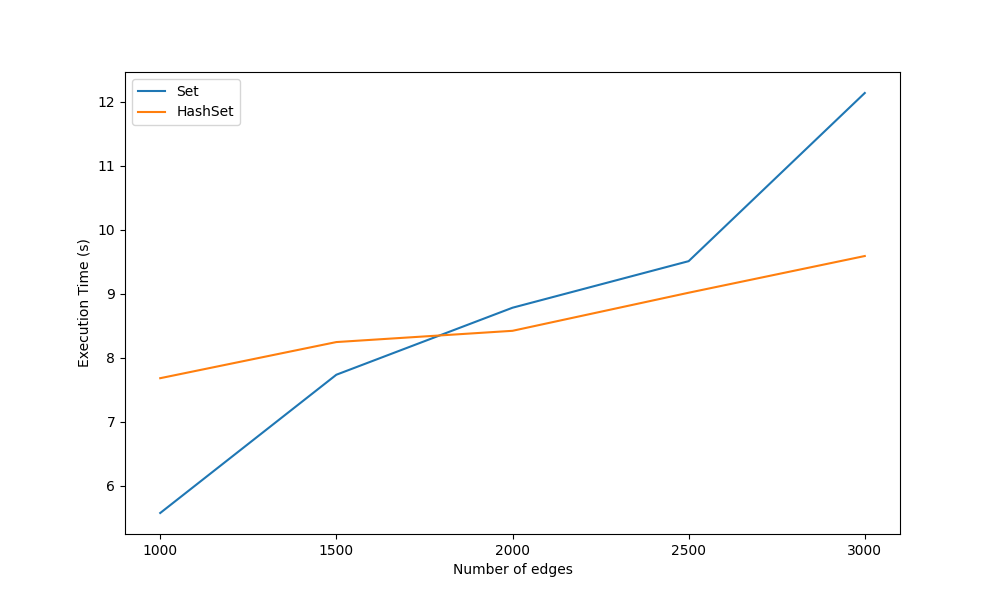
\includegraphics[width=1\textwidth]{ExecutionPlot2.png}
    \caption[{[Exp] Plot Set vs HashSet}]{Plot of execution mean time vs input size for Set and HashSet}
    \label{fig:results6}
\end{figure}

\subsection*{Discussion}
We can see that it seems that we have obtained a performance improvement when the input starts to grow.\\
For smaller inputs, Set obtains better performance, surely because the overhead of making HashSet calculations is high and Set has better performance.
On the other hand, when the input grows, we see how HashSet remains more stable and grows in a more linear way, while Set grows faster due to the overhead of doing the searches.\\

In short, we can conclude that this change has been positive, although it is only for large input types of edges, not for the general case of the algorithm.
\chapter{Conclusions and future work}
In this chapter, we will discuss the conclusions and results of the work. We will also comment on possible future work that could continue this work.
\section{Conclusions}
\section{Future work}
\nocite{*}
\printbibliography
\end{document}